\subsection{Appearance of Period-adding-like structures}
\label{sec:add.change.appa}

\todo{Repeat what was done in last section: first explain how cod-2 point is created, then movement and completion.}

This section explores the appearance of the \gls{pal} structures in between the chains of the same period.
This happens at the horizontal boundaries between ``type A'' parameter regions of different chains, as well as at the vertical boundaries.
The \gls{pal} structures in-between vertically neighboring ``type A'' parameter regions is examined first.
After that the \gls{pal} structures in-between horizontally neighboring ``type A'' parameter regions is examined.

\subsubsection{\Glsentrylong{pal} Structures In-between Vertically Neighboring ``Type A'' Parameter Regions}
\label{sec:add.change.appa.hor}

In \Cref{fig:add.change.regions.1}, the ``type A'' parameter regions $P^{20}_3$ and $P^{18}_3$, as well as $P^{22}_4$ and $P^{20}_4$ overlap.
This changes in \Cref{fig:add.change.regions.2}.
Here only the ``type A'' parameter regions $P^{20}_3$ and $P^{18}_3$ overlap, the parameter regions $P^{22}_4$ and $P^{20}_4$ stopped overlapping.
Instead, in the space between the two ``type A'' parameter region there are now two asymmetric coexisting twin cycles $\Cycle{\A^8\B^3\C^8\D^2}$ and $\Cycle{\A^8\B^2\C^8\D^3}$.
Those cycles are \textbf{not} ``type B'' cycles, because they only differ in the number of points on the branches $f_\B$ and $f_\D$.
Remember that ``type B'' cycles are asymmetrical twin cycles $\Cycle{\A^a\B^b\C^c\D^d}$ and $\Cycle{\A^c\B^d\C^a\D^b}$ where $c = a - 1$ and $d = b + 1$.
This is not the case here, since $a = c$.
Instead, we will call them hybrid cycles and ``type B'' cycles are a special case of hybrid cycles.
The notation $\left[P^{22}_4 \mid P^{20}_4\right]$ used in the diagrams was introduced in \Cref{sec:add.change.num} and is formally defined later in \Cref{sec:add.add.halved}.
Later in \Cref{fig:add.change.regions.4}, the ``type A'' parameter regions $P^{20}_3$ and $P^{18}_3$ also stop overlapping.
In between, there are also hybrid cycles, $\Cycle{\A^7\B^3\C^6\D^3}$ and $\Cycle{\A^6\B^3\C^7\D^3}$.
This parameter region is therefore labeled $\left[P^{20}_3 \mid P^{18}_3\right]$.

\begin{figure}
	\centering
	\subfloat[Regions]{
		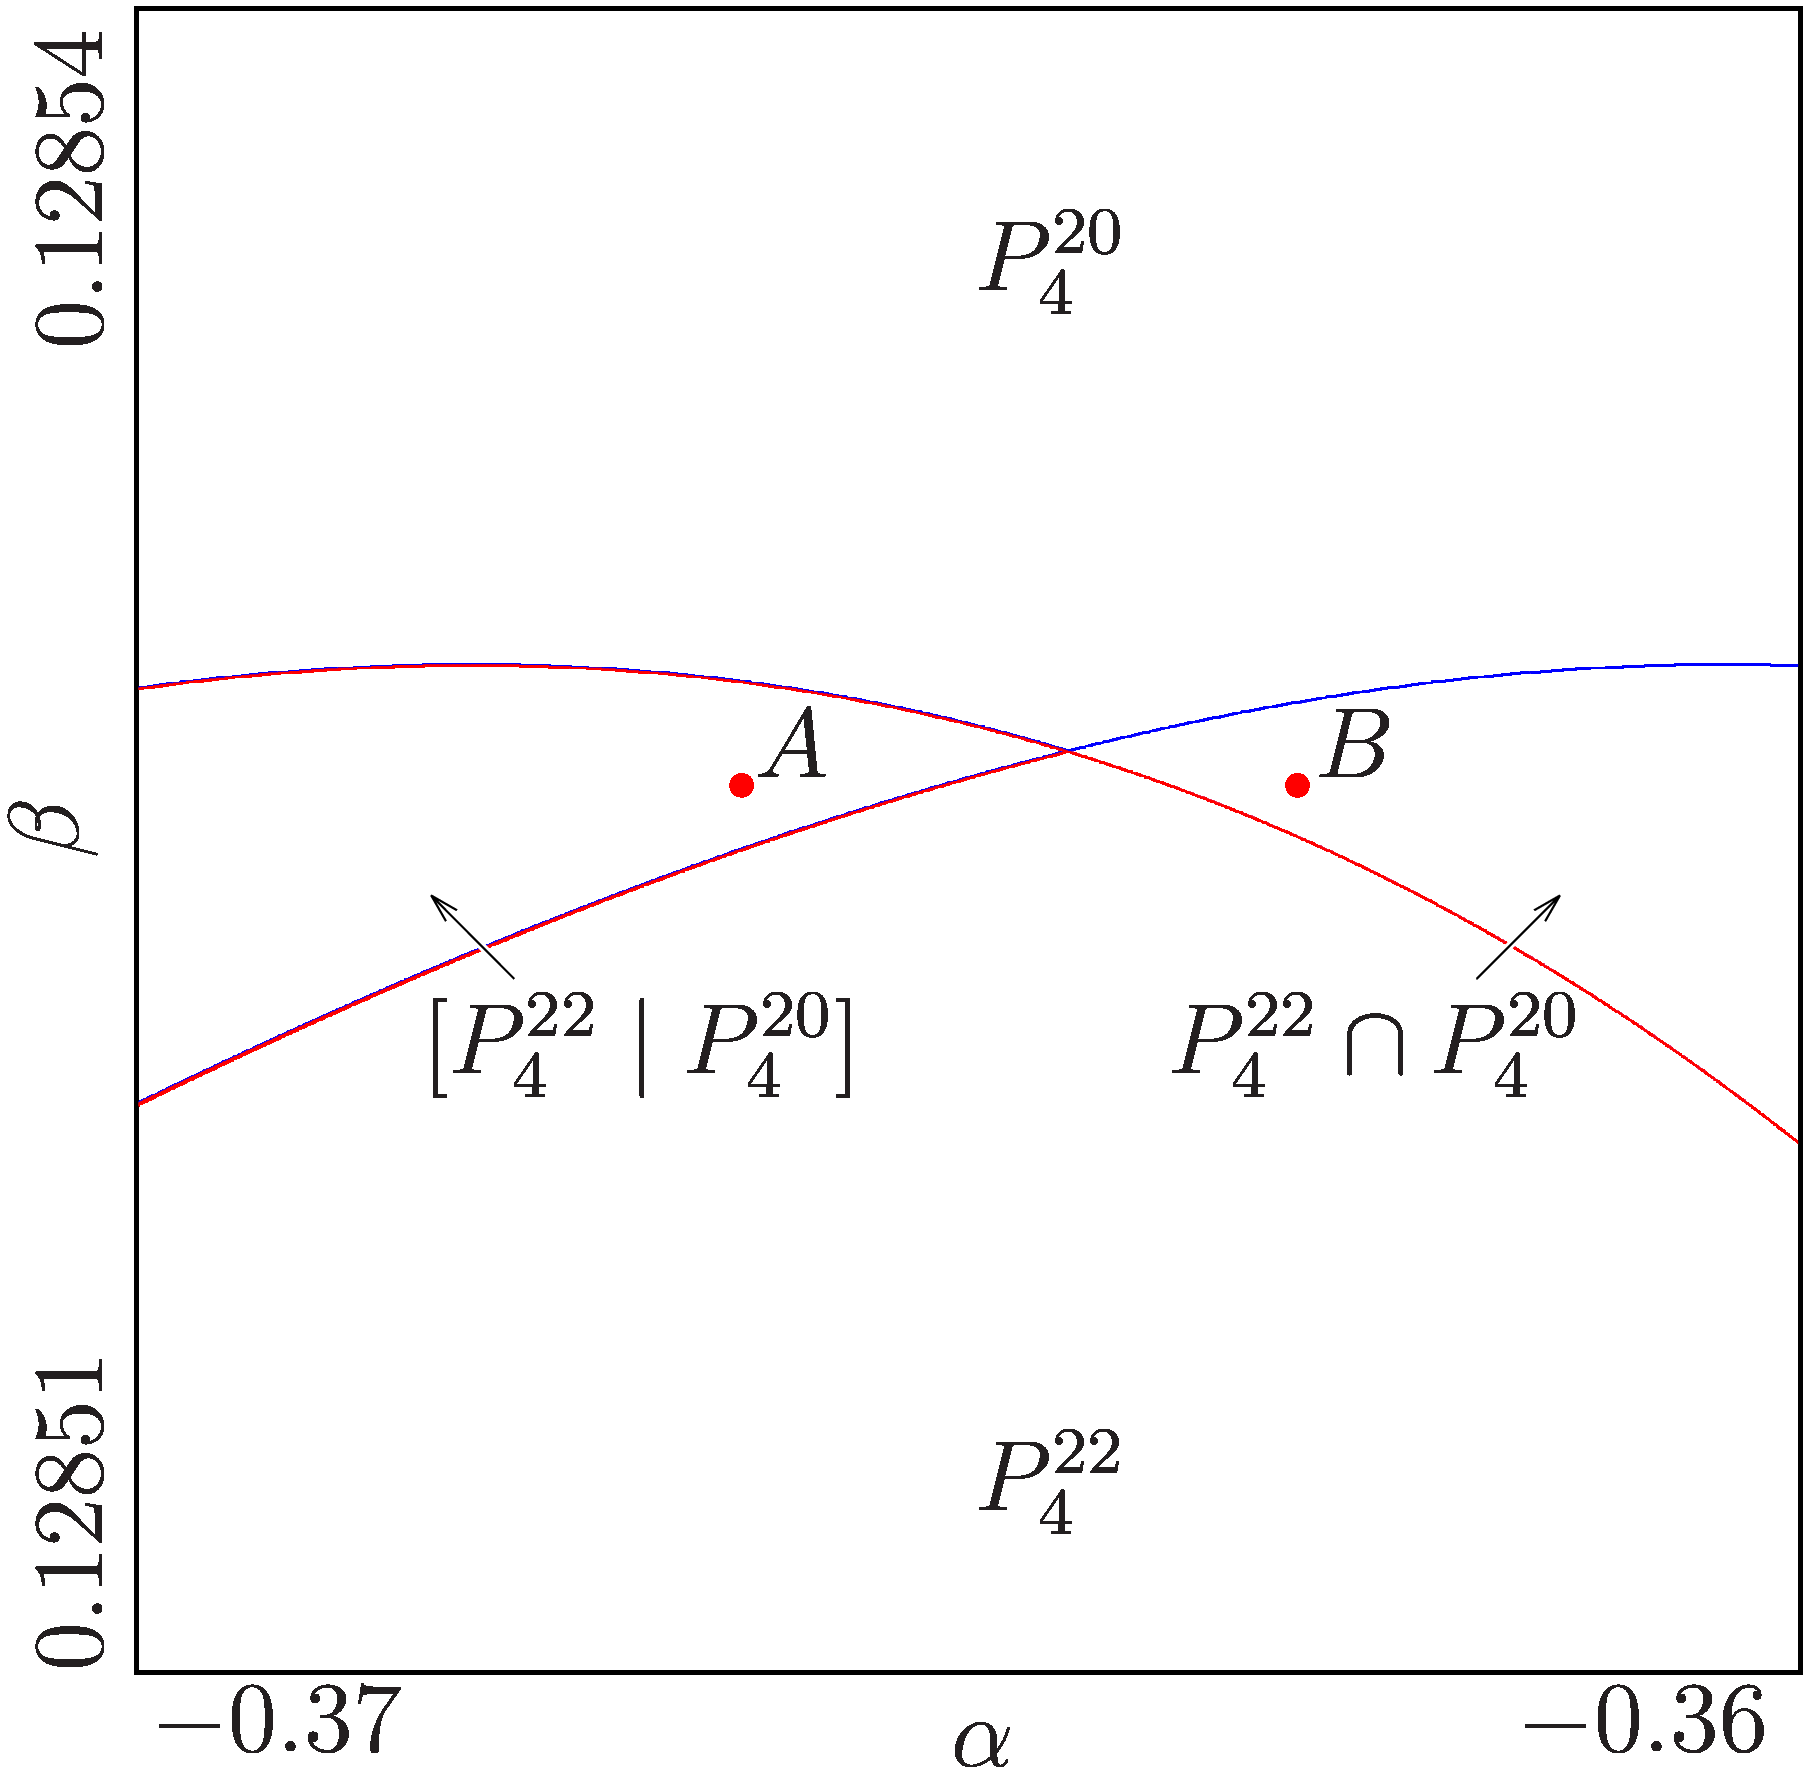
\includegraphics[width=.3 \textwidth]{../Figures/7/7.5a/result.png}
		\label{fig:add.change.appa.hor.regions}
	}
	\subfloat[At point $A$]{
		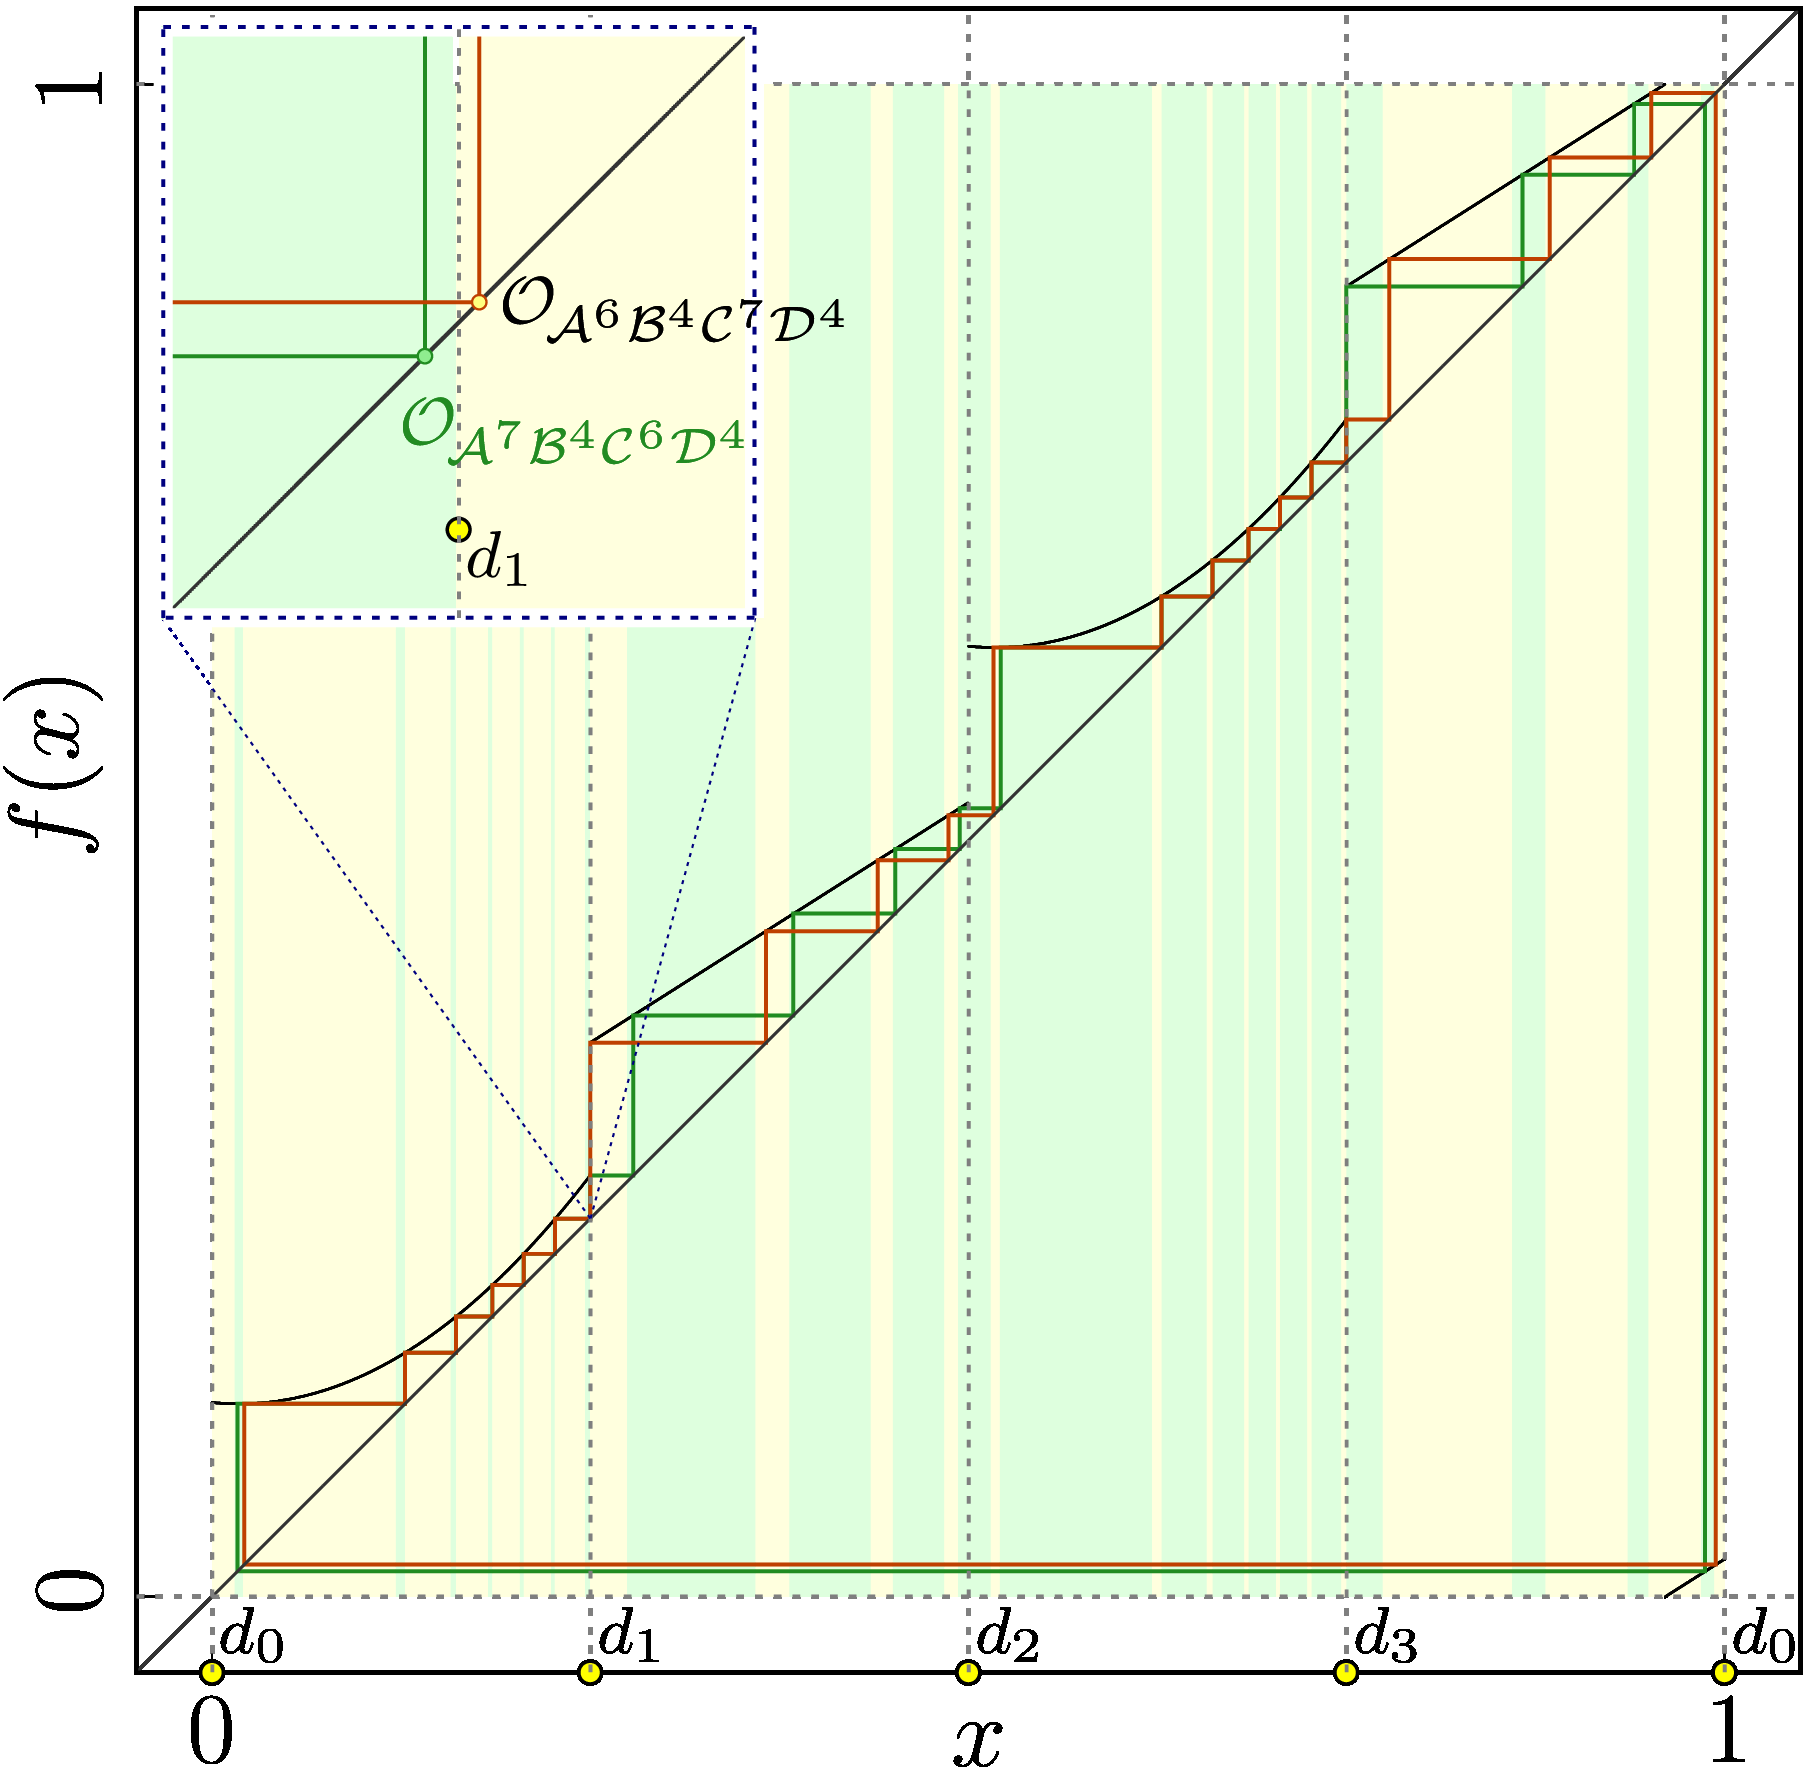
\includegraphics[width=.3 \textwidth]{../Figures/7/7.5b/result.png}
		\label{fig:add.change.appa.hor.cob.A}
	}
	\subfloat[At point $B$]{
		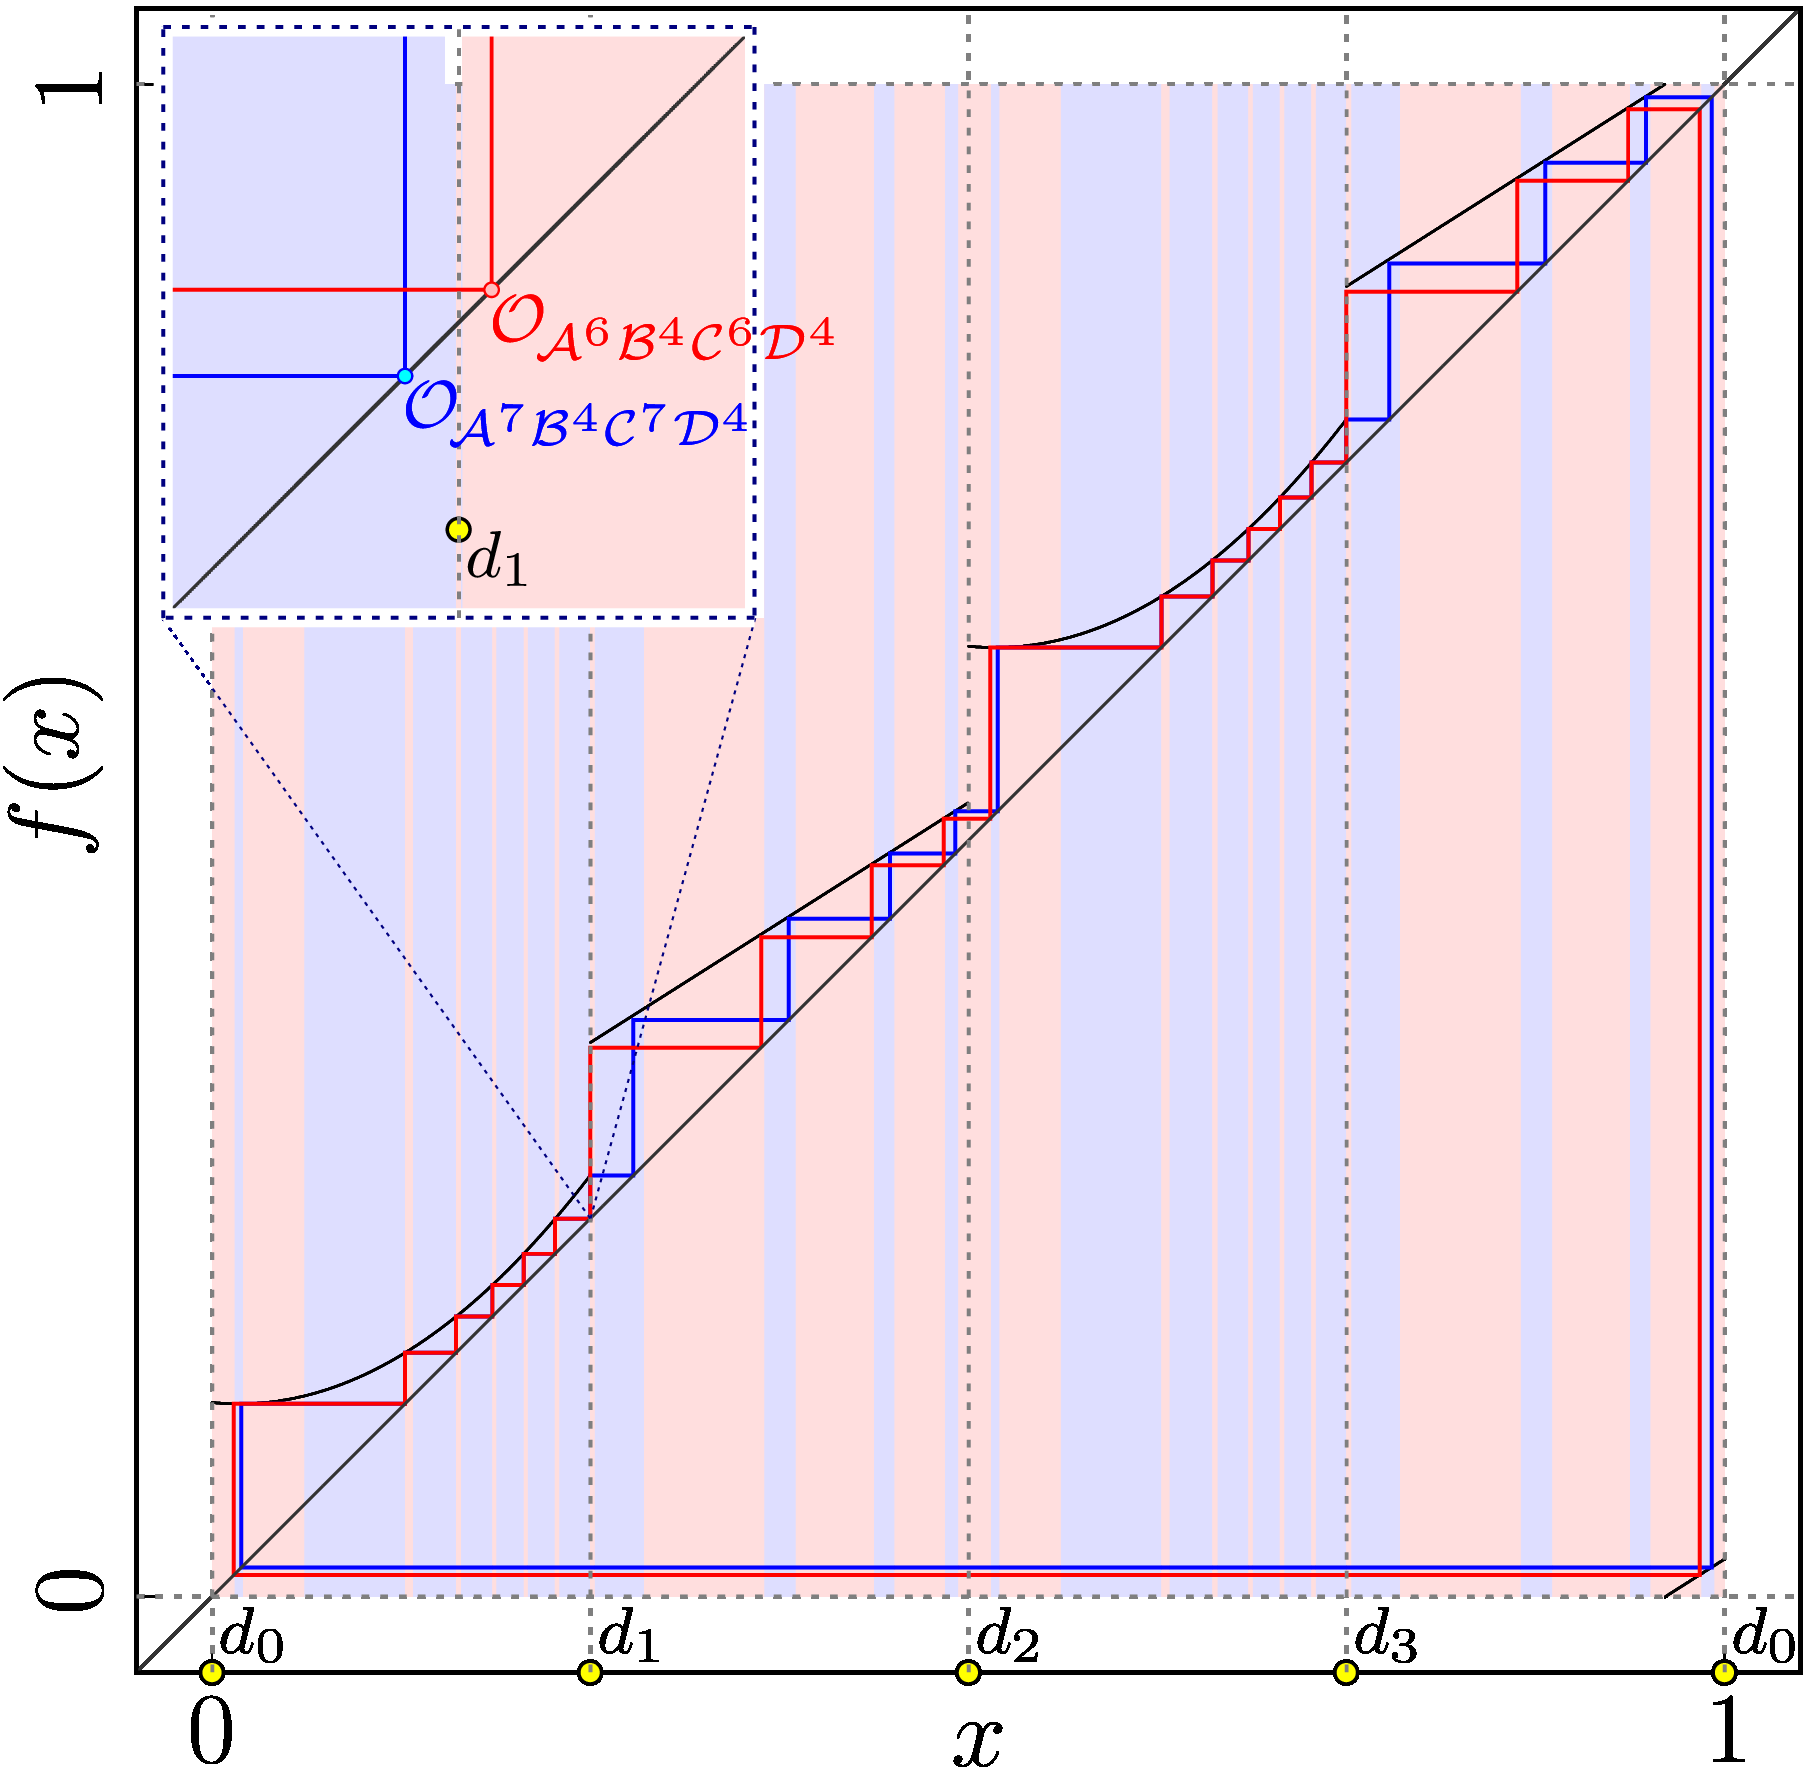
\includegraphics[width=.3 \textwidth]{../Figures/7/7.5c/result.png}
		\label{fig:add.change.appa.hor.cob.B}
	}
	\caption[2D boundary scan and cobweb diagrams showing the appearance of horizontal period-adding-like structures in the archetypal model]{
		2D boundary scan and cobweb diagrams showing the appearance of horizontal period-adding-like structures in the archetypal model.
		The parameters $a_L = 2.8, b_L = -0.1,$ and $g_R\left(\frac{1}{2}\right) = \frac{1}{2} + \frac{1}{40}$ are fixed.
		(a) shows a boundary scan of parameter regions associated with different symbolic sequences.
		The parameters $\alpha = g_R\left(\frac{1}{4}\right)$ and $\beta = c_L$ are varied.
		(b) and (c) show the cobweb diagrams at the parameter values marked with the points $A$ and $B$ in (a).
	}
\end{figure}

For some parameter values along the line given by \Cref{equ:add.change.paramline} between the parameter values used for \Cref{fig:add.change.regions.1,fig:add.change.regions.2}, upper left corner of $P^{22}_4$ crosses the lower boundary of $P^{20}_4$.
This causes the boundaries of $P^{22}_4$ and $P^{20}_4$ to cross, similar to the last section where the boundaries of $P^{20}_3$ and $P^{20}_4$ started overlapping.
But in this case, the overlapping parameter region $P^{22}_4 \cap P^{20}_4$ had four boundaries before and now has only three boundaries with the point where the boundaries cross moving right.
The point where the boundaries cross cannot be seen in \Cref{fig:add.change.regions.2}, but it is visible in \Cref{fig:add.change.appa.hor.regions}.
We know from \Cref{sec:arch.bif.sum} that the border collision bifurcation at the upper boundary of the ``type A'' parameter region $P^{22}_4$ is $\BCB_{d_1, d_3}^{\underline{\A}^7\B^4\underline{\C}^7\D^4}$.
And the border collision bifurcation at the lower boundary of the ``type A'' parameter region $P^{20}_4$ is $\BCB_{d_1, d_3}^{\A^6\underline{\B}^4\C^6\underline{\D}^4}$.
Both these border collision bifurcations are at the upper and lower boundaries of the overlapping region $P^{22}_4 \cap P^{20}_4$.
At the point where these boundaries cross, both these border collision bifurcations happen at the same time and both cycles vanish.
We can see in \Cref{fig:add.change.appa.hor.cob.A} that the ``type A'' cycles are very close to the borders $d_1$ and $d_3$, respectively.

Similarly, the hybrid parameter region $\left[P^{22}_4 \mid P^{20}_4\right]$ that emerged in the opening space has a codimension-2 point as its right corner.
Just as the ``type B'' parameter region had a codimension-2 point as its left corner.
\Cref{fig:add.change.appa.hor.cob.A} shows the coexisting hybrid cycles in this hybrid parameter region.
And \Cref{fig:add.change.appa.hor.bif.lower,fig:add.change.appa.hor.bif.upper} show the border collision bifurcations at the upper and lower boundaries of the hybrid parameter region, $\BCB_{d_3}^{\A^7\B^4\C^6\underline{\D}^4}$ and $\BCB_{d_1}^{\A^6\underline{\B}^4\C^7\D^4}$ at the lower boundary and $\BCB_{d_1}^{\underline{\A}^7\B^4\C^6\D^4}$ and $\BCB_{d_3}^{\A^6\B^4\underline{\C}^7\D^4}$ at the upper boundary.
Those four border collision bifurcations happen at the codimension-2 point.
Again, the coexisting hybrid twin cycles are very close to the borders $d_1$ and $d_3$ for the parameter values marked with the point $B$ in \Cref{fig:add.change.appa.hor.regions}.
We can see this in the cobweb diagram in \Cref{fig:add.change.appa.hor.cob.B}.

\begin{figure}
	\centering
	\subfloat[Lower boundary]{
		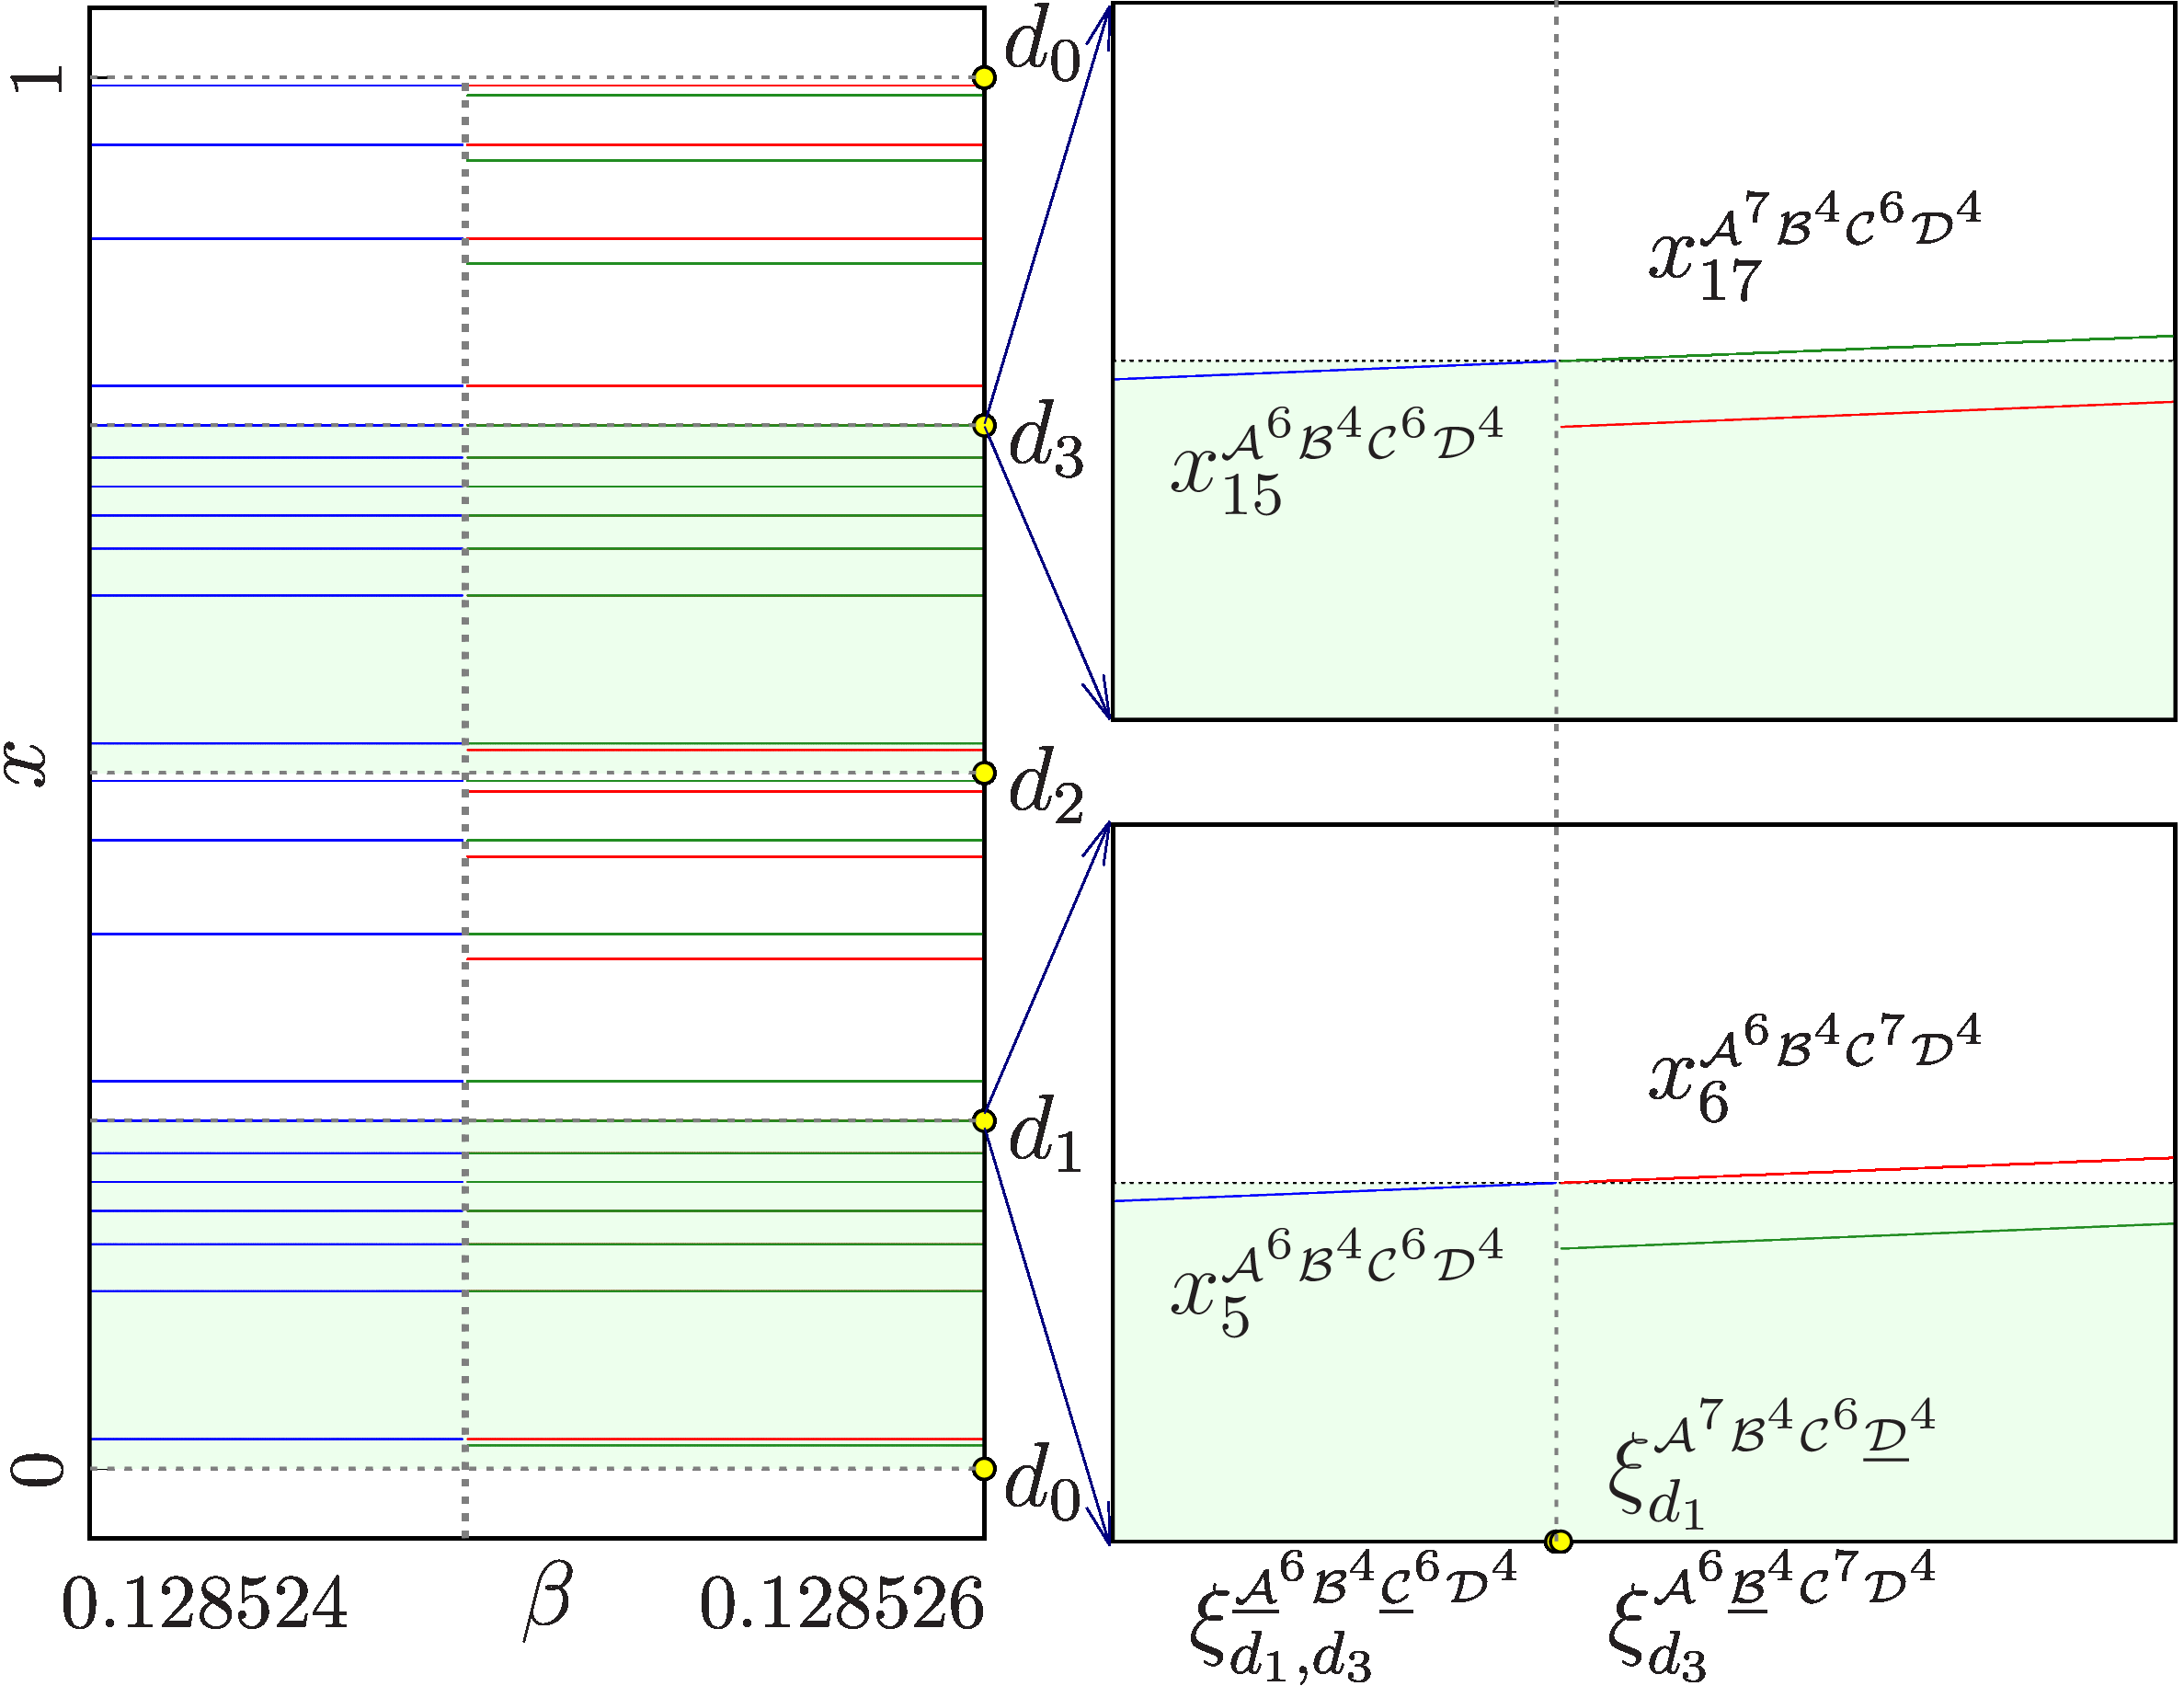
\includegraphics[width=.45 \textwidth]{../Figures/7/7.6a/result.png}
		\label{fig:add.change.appa.hor.bif.lower}
	}
	\subfloat[Upper boundary]{
		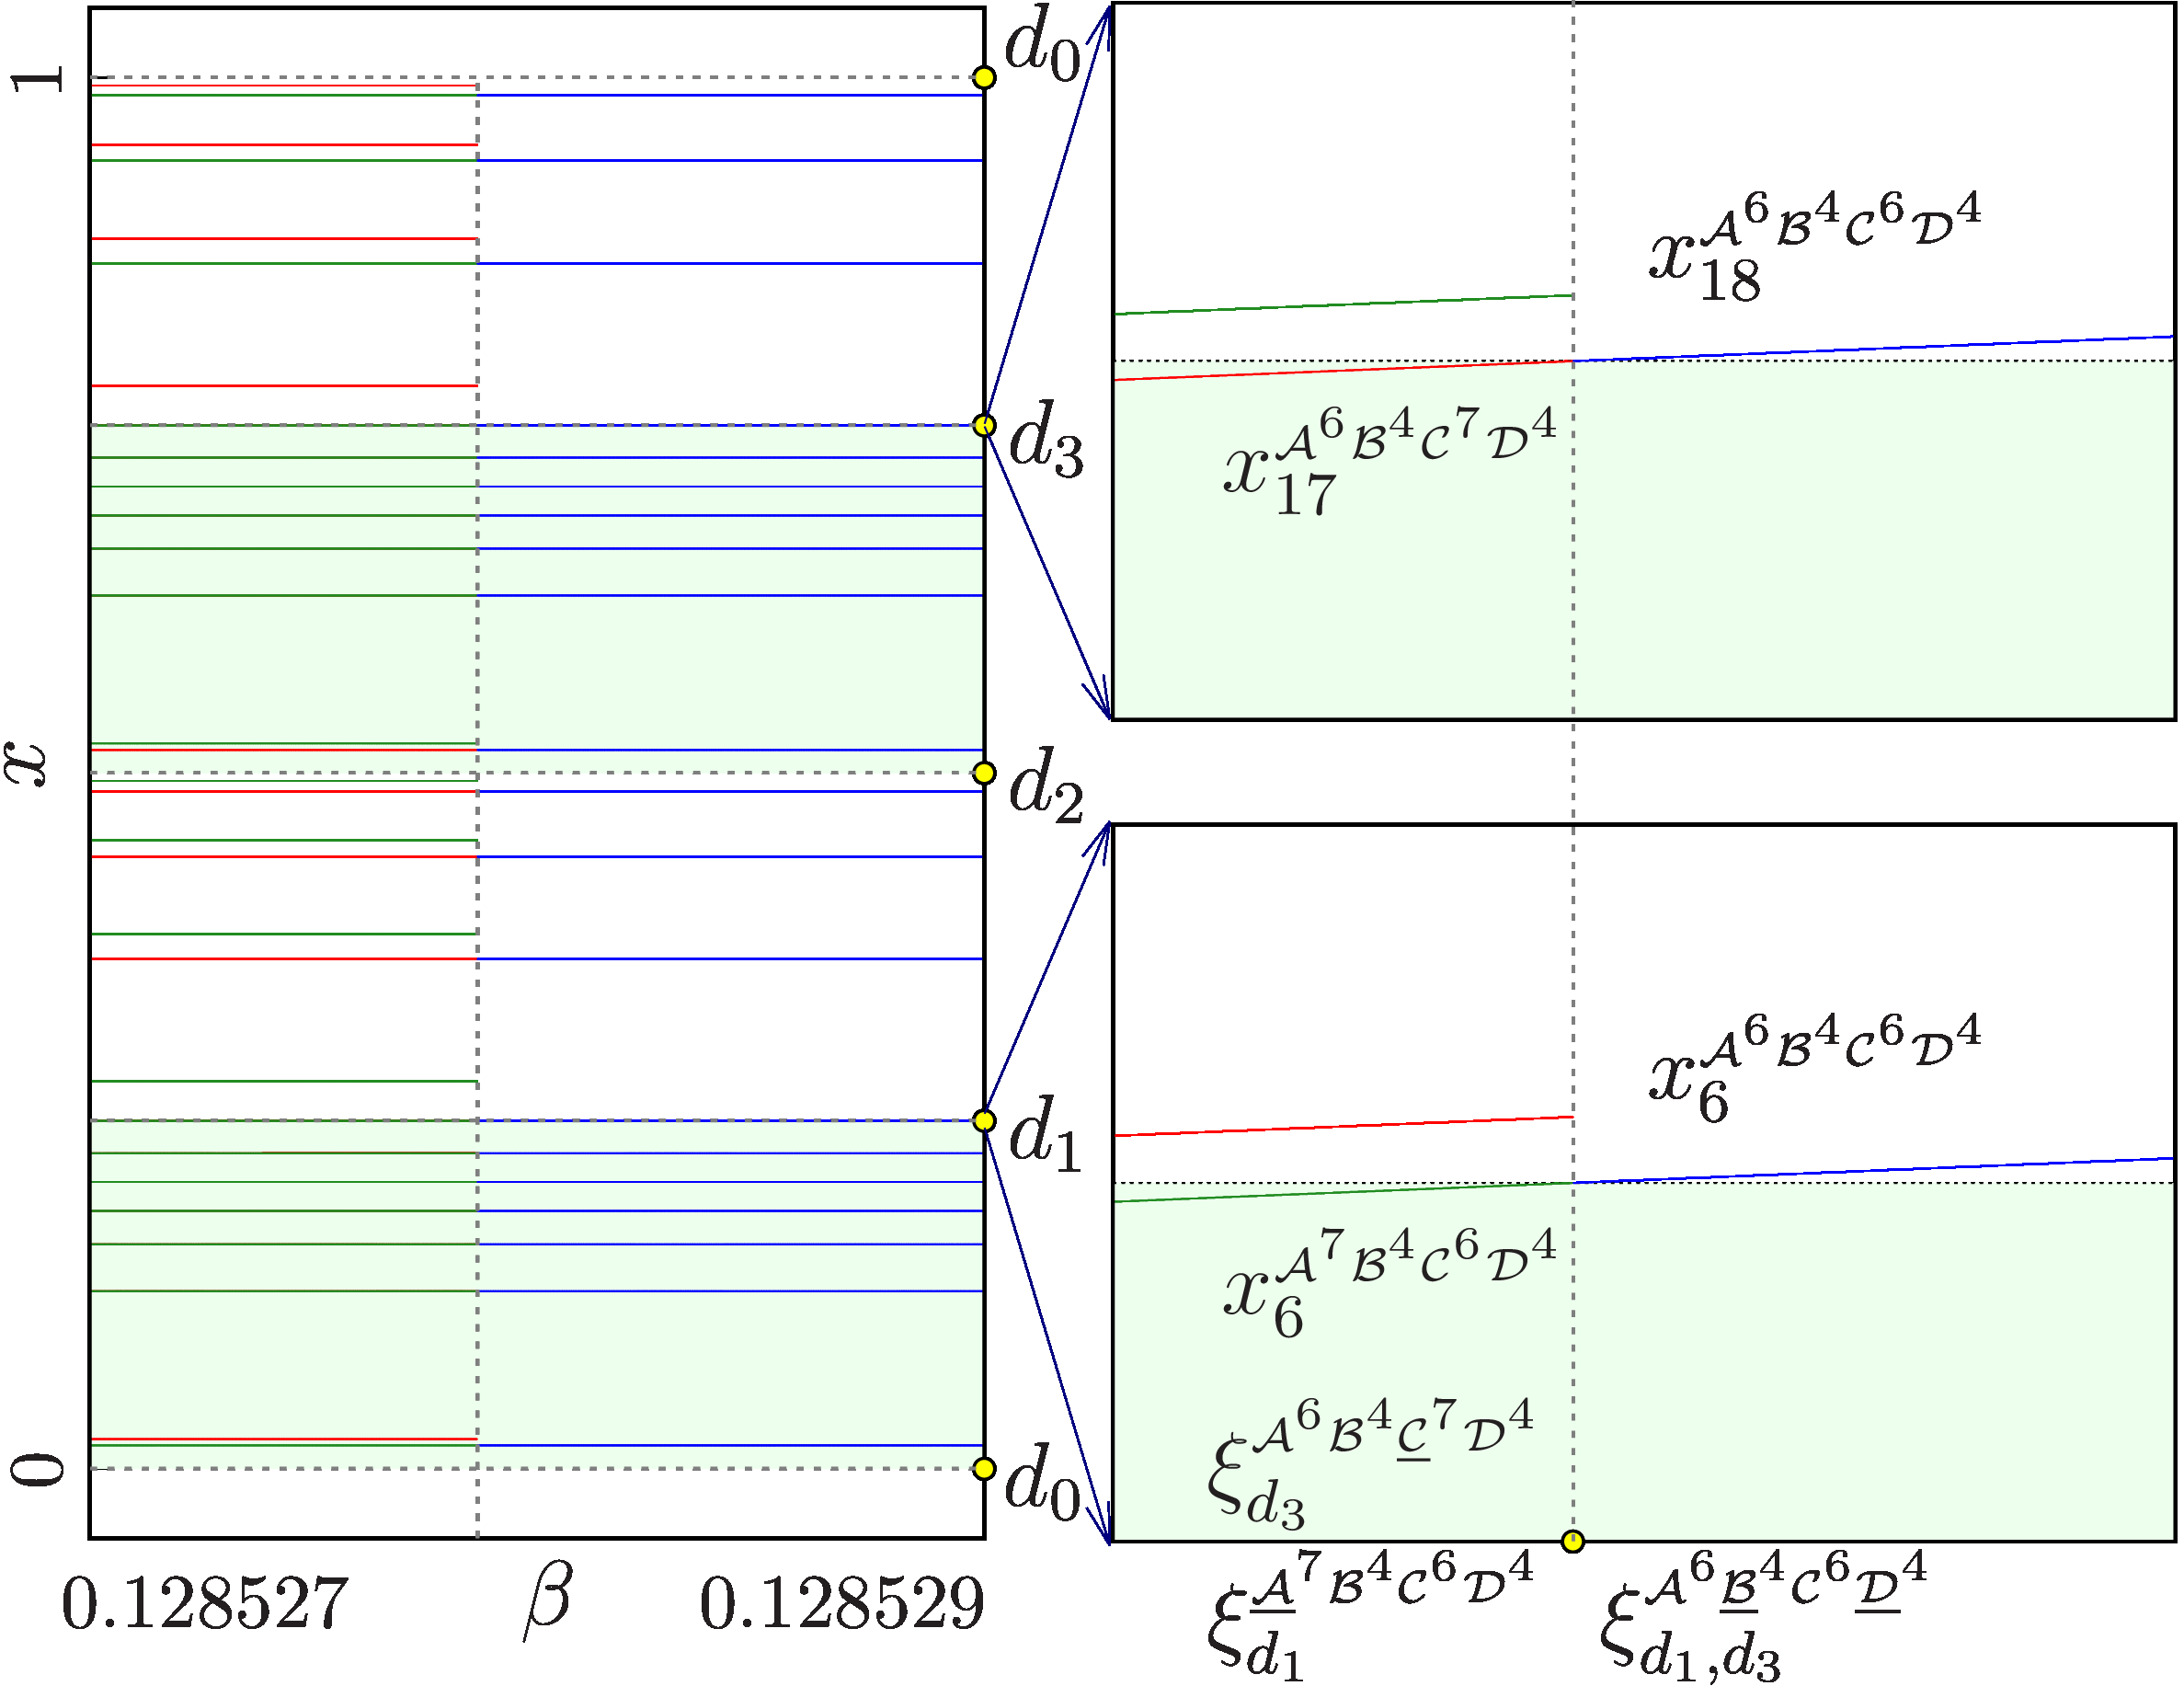
\includegraphics[width=.45 \textwidth]{../Figures/7/7.6b/result.png}
		\label{fig:add.change.appa.hor.bif.upper}
	}
	\caption[Bifurcation diagrams for the horizontal hybrid parameter regions in the increasing archetypal model]{
		Bifurcation diagrams at the horizontal boundaries of the horizontal hybrid parameter region $\left[P^{22}_4 \mid P^{20}_4\right]$.
		The parameters $a_L = 2.8, b_L = -0.1, g_R\left(\frac{1}{2}\right) = \frac{1}{2} + \frac{1}{40},$ and $\alpha = g_R\left(\frac{1}{4}\right) = 0.366362$ are fixed.
		The parameter $\beta = c_L$ is varied.
		(a) shows the bifurcation diagram at the lower boundary, while (b) shows the bifurcation diagram at the upper boundary.
	}
	\label{fig:add.change.appa.hor.bif}
\end{figure}

Both corner points move right for increasing values of $b_L$ along the parameter line given by \Cref{equ:add.change.paramline}.
This is again caused by the movement of the boundaries of the ``type A'' parameter regions and the hybrid parameter region $\left[P^{22}_4 \mid P^{20}_4\right]$.
This time, the overlapping area disappears as soon as its left corner collides with the lower right corner of $P^{20}_4$ and the upper right corner of $P^{22}_4$.
And the hybrid parameter region has four boundaries as soon as its corner point reaches the theoretical right boundary.
This transition can be seen for the parameter regions $P^{20}_3$ and $P^{18}_3$ in \Cref{fig:add.change.regions.1,fig:add.change.regions.4}.

The appearance of the hybrid parameter region and the \gls{pal} structures in-between vertically neighboring ``type A'' parameter regions is very similar to the disappearance of ``type B'' parameter regions described in \Cref{sec:add.change.disb}.
But instead of the overlapping parameter region of two ``type A'' parameter regions appearing, it disappeared and a parameter region with two coexisting asymmetrical twin cycles appeared instead of disappearing.

\subsubsection{\Glsentrylong{pal} Structures In-between Horizontally Neighboring ``Type A'' Parameter Regions}
\label{sec:add.change.appa.vert}

In contrast to the \gls{pal} structures in-between vertically neighboring ``type A'' parameter region, no numerical evidence for a crossing of boundaries of ``type A'' parameter regions could be found.
As far as this thesis is concerned, the opening of the space between horizontally neighboring ``type A'' parameter regions happens at once.

In \Crefrange{fig:add.change.regions.1}{fig:add.change.regions.3}, the parameter regions $P^{20}_3$ and $P^{22}_4$, as well as $P^{18}_3$ and $P^{20}_4$ overlap.
And in \Cref{fig:add.change.regions.4} they do not overlap, instead there is space in-between these vertically neighboring ``type A'' parameter regions with hybrid parameter regions and \gls{pal} structures.
The appearance of the parameter region $\left[P^{20}_3 \mid P^{22}_4\right]$ in between $P^{20}_3$ and $P^{22}_4$ seems to happen at the same time as the appearance of the hybrid parameter region $\left[P^{18}_3 \mid P^{20}_4\right]$ in between $P^{18}_3$ and $P^{20}_4$, at some parameter values on the line given by \Cref{equ:add.change.paramline} between the parameter values of \Cref{fig:add.change.regions.3,fig:add.change.regions.4}.
And with these hybrid parameter regions the vertical period-adding-like structures between them and the neighboring ``type A'' parameter regions also appear.

\Cref{fig:add.change.appa.vert.regions.A,fig:add.change.appa.vert.regions.B} show this transition again for the parameter regions $P^{20}_3$ and $P^{22}_4$.
As mentioned before, we assume that there is no crossing of the boundaries of the ``type A'' parameter regions in a point that moves up or down as in the previous section.
This means that at some parameter values, the boundaries are perfectly aligned with the ``type A'' parameter regions overlapping for values on the parameter line for smaller values $b_L$ and a hybrid parameter region for lager values of $b_L$.

\begin{figure}
	\centering
	\subfloat[With $a_L = 2.8, b_L = -0.1$]{
		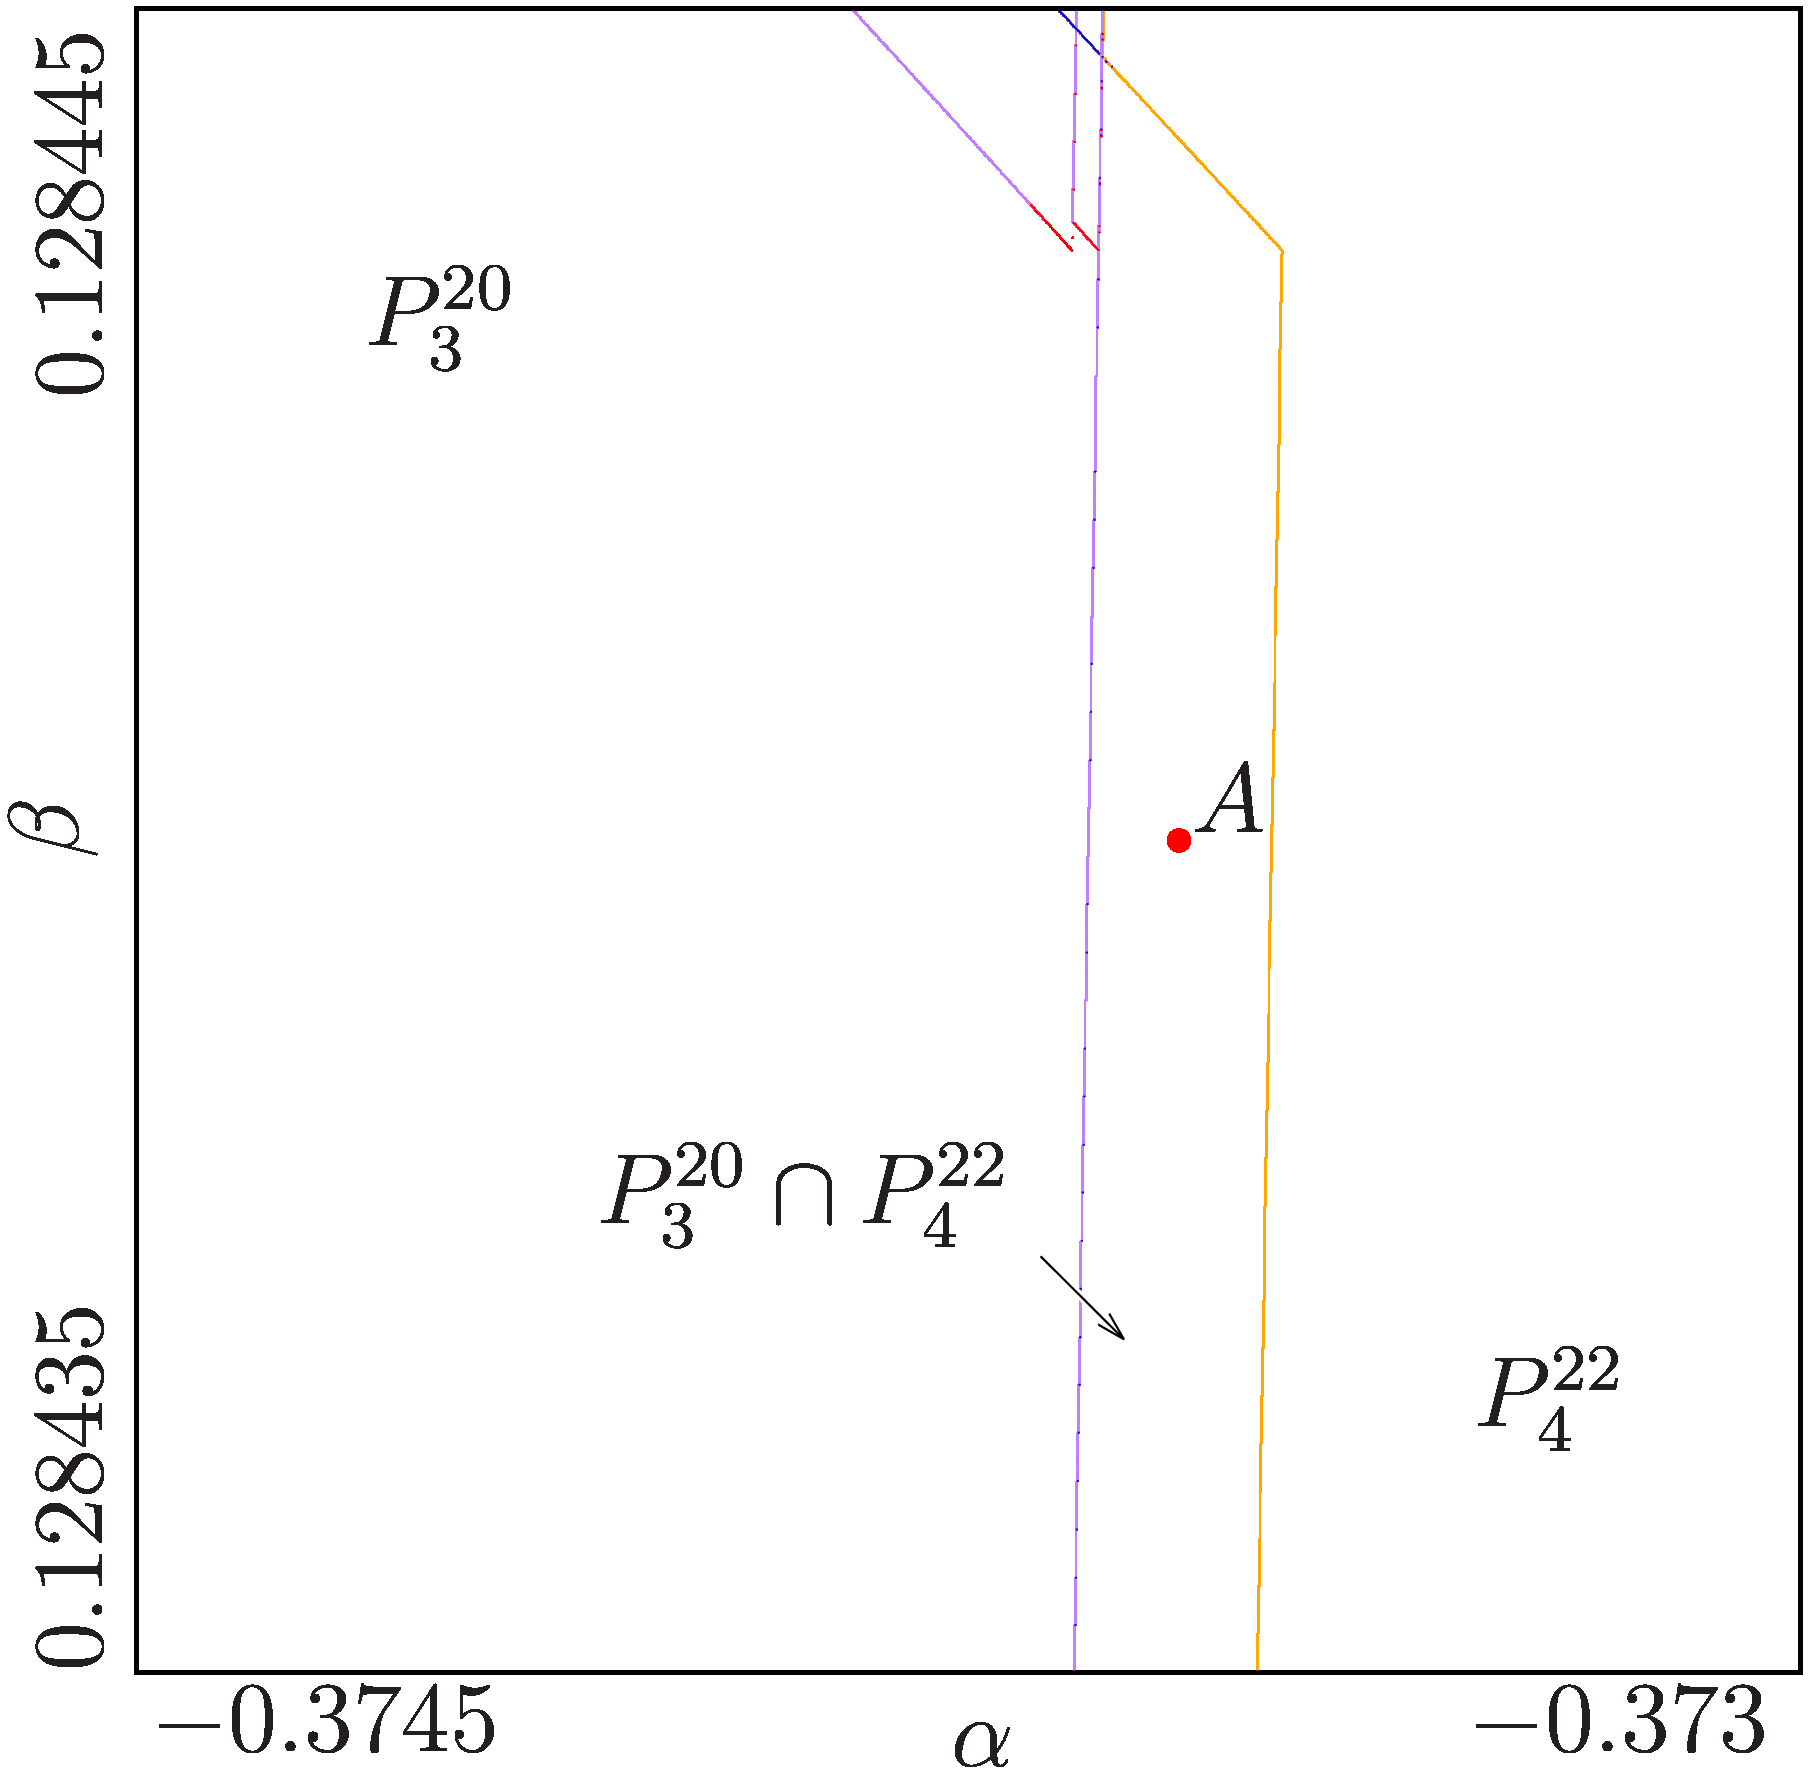
\includegraphics[width=.4 \textwidth]{../Figures/7/7.7a/result.png}
		\label{fig:add.change.appa.vert.regions.A}
	}
	\subfloat[With $a_L = 2.65, b_L = -0.05$]{
		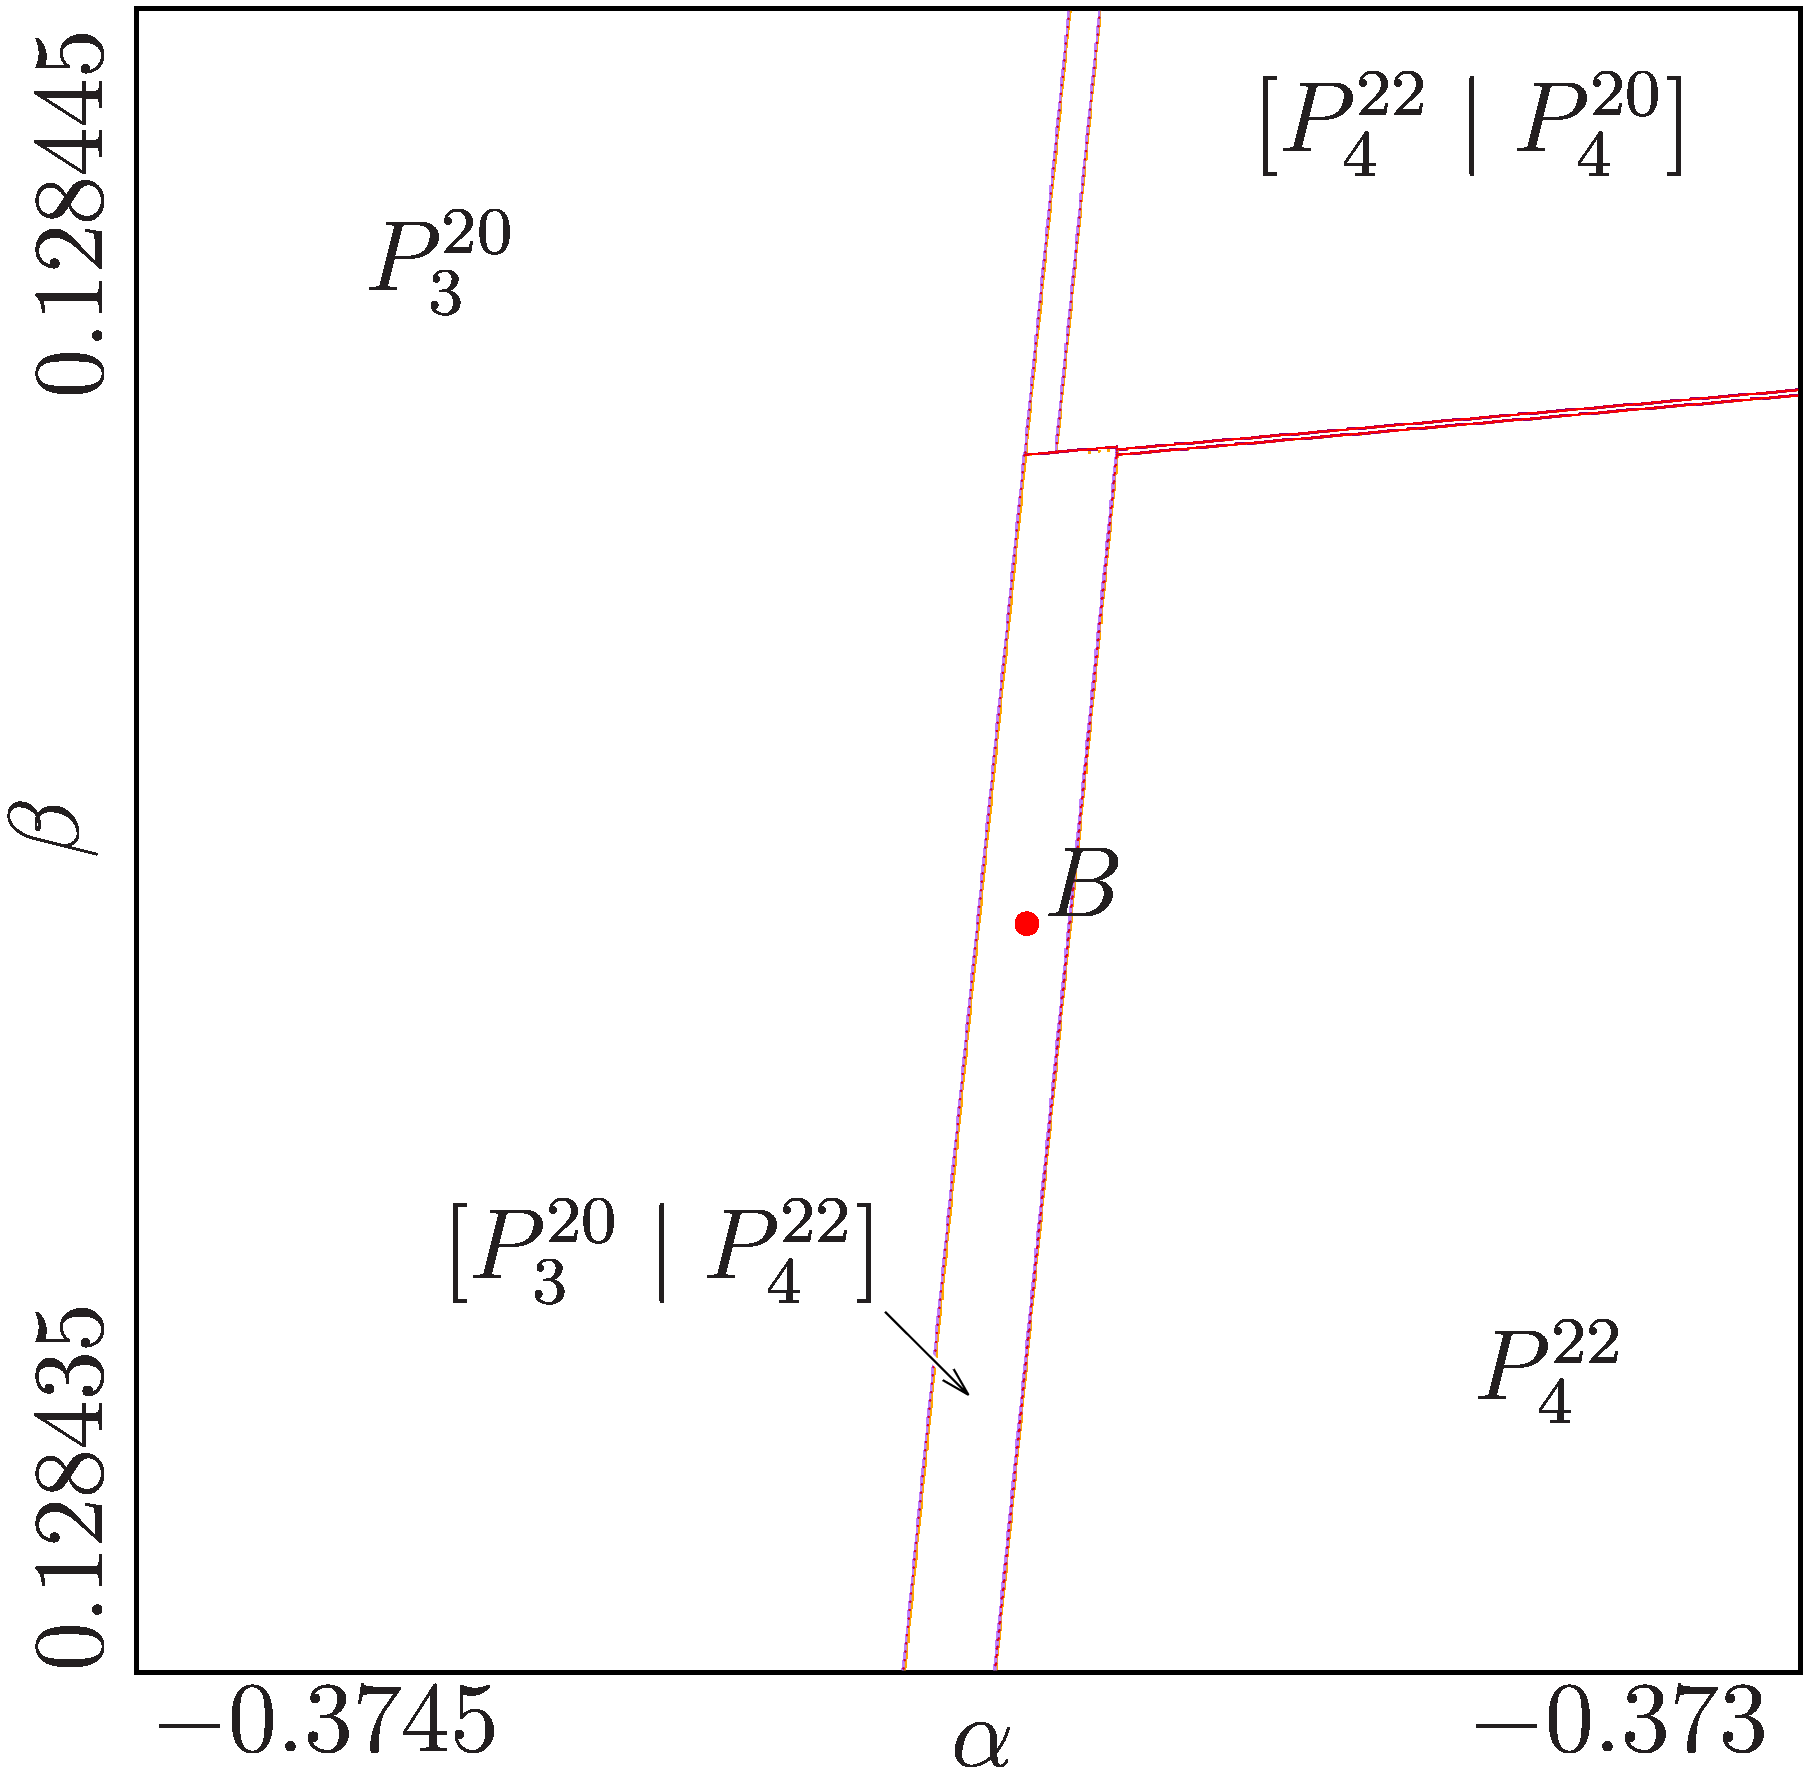
\includegraphics[width=.4 \textwidth]{../Figures/7/7.7b/result.png}
		\label{fig:add.change.appa.vert.regions.B}
	} \\
	\subfloat[At point $A$]{
		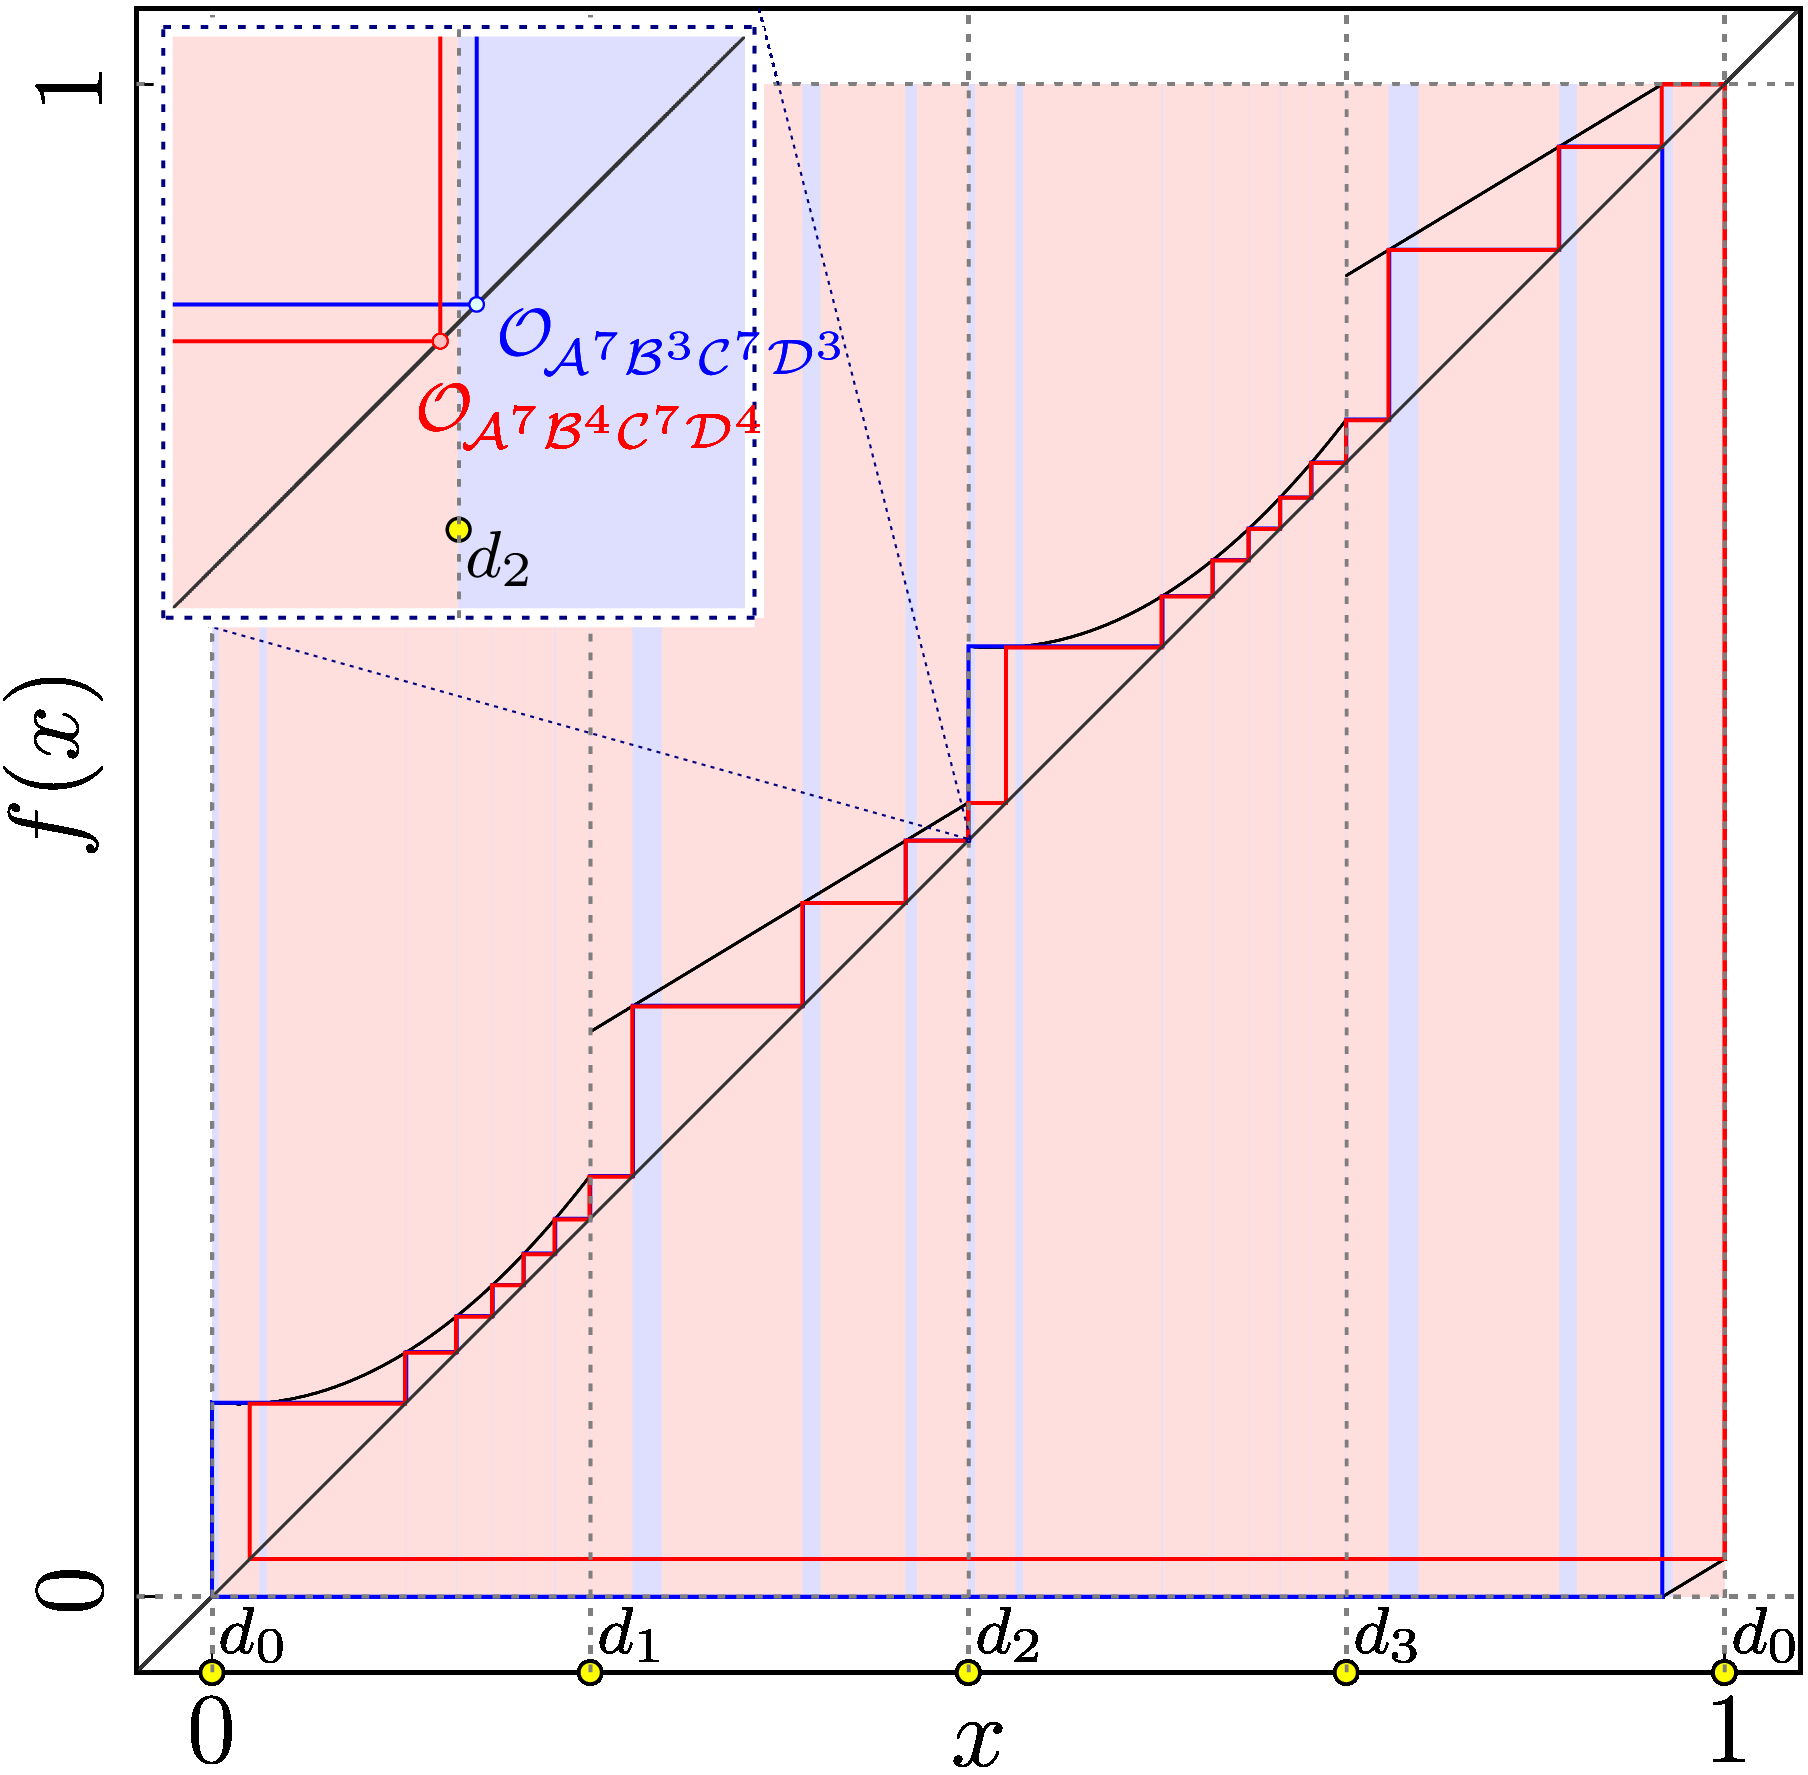
\includegraphics[width=.4 \textwidth]{../Figures/7/7.7c/result.png}
		\label{fig:add.change.appa.vert.cobweb.A}
	}
	\subfloat[At point $B$]{
		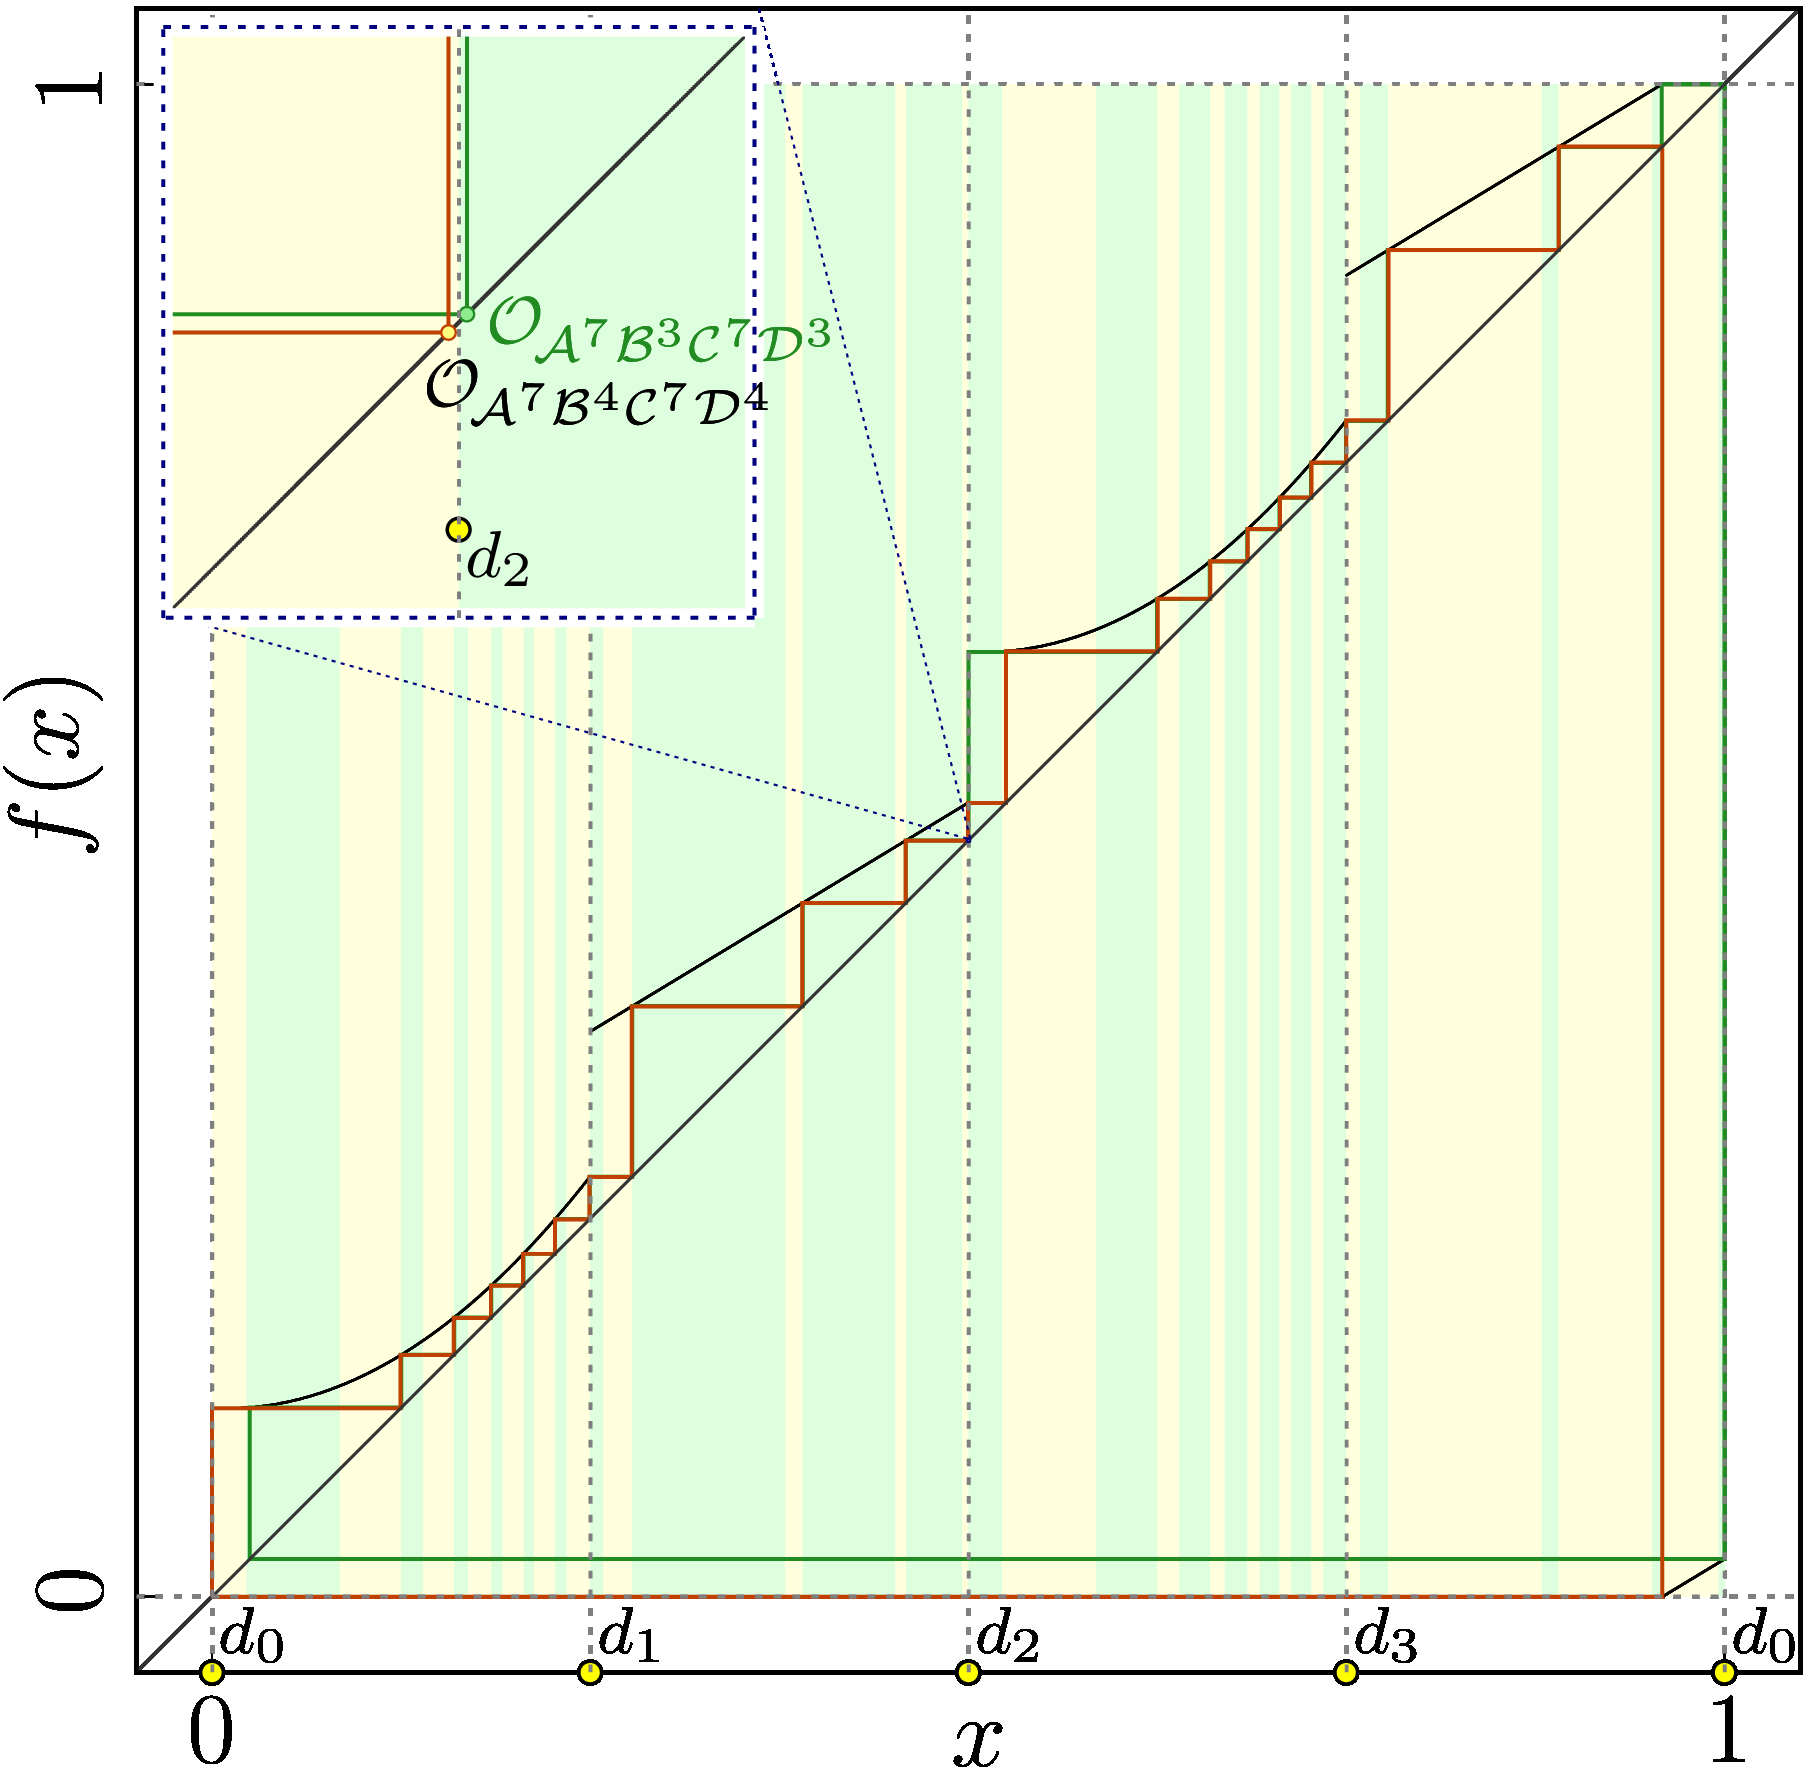
\includegraphics[width=.4 \textwidth]{../Figures/7/7.7d/result.png}
		\label{fig:add.change.appa.vert.cobweb.B}
	}
	\caption[2D boundary scans and cobweb diagrams showing the appearance of vertical period-adding-like structures in the archetypal model]{
		2D boundary scans and cobweb diagrams showing the appearance of vertical period-adding-like structures in the archetypal model.
		The parameter $g_R\left(\frac{1}{2}\right) = \frac{1}{2} + \frac{1}{40}$ is fixed for all diagrams.
		(a) and (b) show boundary scans of parameter regions associated with different symbolic sequences.
		The parameters $a_L$ and $b_L$ are fixed in each 2D boundary scan, with the values given in the sub-captions.
		The parameters $\alpha = g_R\left(\frac{1}{4}\right)$ and $\beta = c_L$ are varied.
		(c) and (d) show cobweb diagrams at the parameter values marked with points $A$ and $B$ in (a) and (b), respectively.
	}
\end{figure}

\Cref{fig:add.change.appa.vert.cobweb.A} shows the coexistence of the two coexisting ``type A'' cycles while the ``type A'' parameter regions still overlap.
\Cref{fig:add.change.appa.vert.cobweb.B} shows the coexistence of the two coexisting hybrid cycles in the newly created parameter region $\left[P^{20}_3 \mid P^{22}_4\right]$.
In both cases, the coexisting cycles are very close to the borders $d_0$ and $d_2$.

The border collision bifurcations at the left and right boundary of the hybrid parameter region follow the same rules as the border collision bifurcations ``type B'' parameter regions.
At the left boundary, the hybrid cycles collide with the borders $d_0$ and $d_2$ from the left at the same time, pictured in \Cref{fig:add.appa.vert.bif.left}.
And at the right boundary, they collide with the same borders from the right at the same time, pictured in \Cref{fig:add.appa.vert.bif.right}.
Note that at the left boundary, the border collision bifurcations of the hybrid cycles are left of the border collision bifurcation of the ``type A'' cycle.
This causes all three cycles to coexist in the parameter region between the border collision bifurcations.
At the right boundary on the other hand, the border collision bifurcations of the hybrid cycles are also left of the border collision bifurcation of the ``type A'' cycle.
This causes a space between the hybrid parameter region $\left[P^{20}_3 \mid P^{22}_4\right]$ and the ``type A'' parameter region $P^{20}_3$ where a period-adding-like structure emerges.
The cycle of the first stage of this period-adding-like structure is visible in purple in \Cref{fig:add.appa.vert.bif.right}.

\begin{figure}
	\centering
	\subfloat[Left boundary]{
		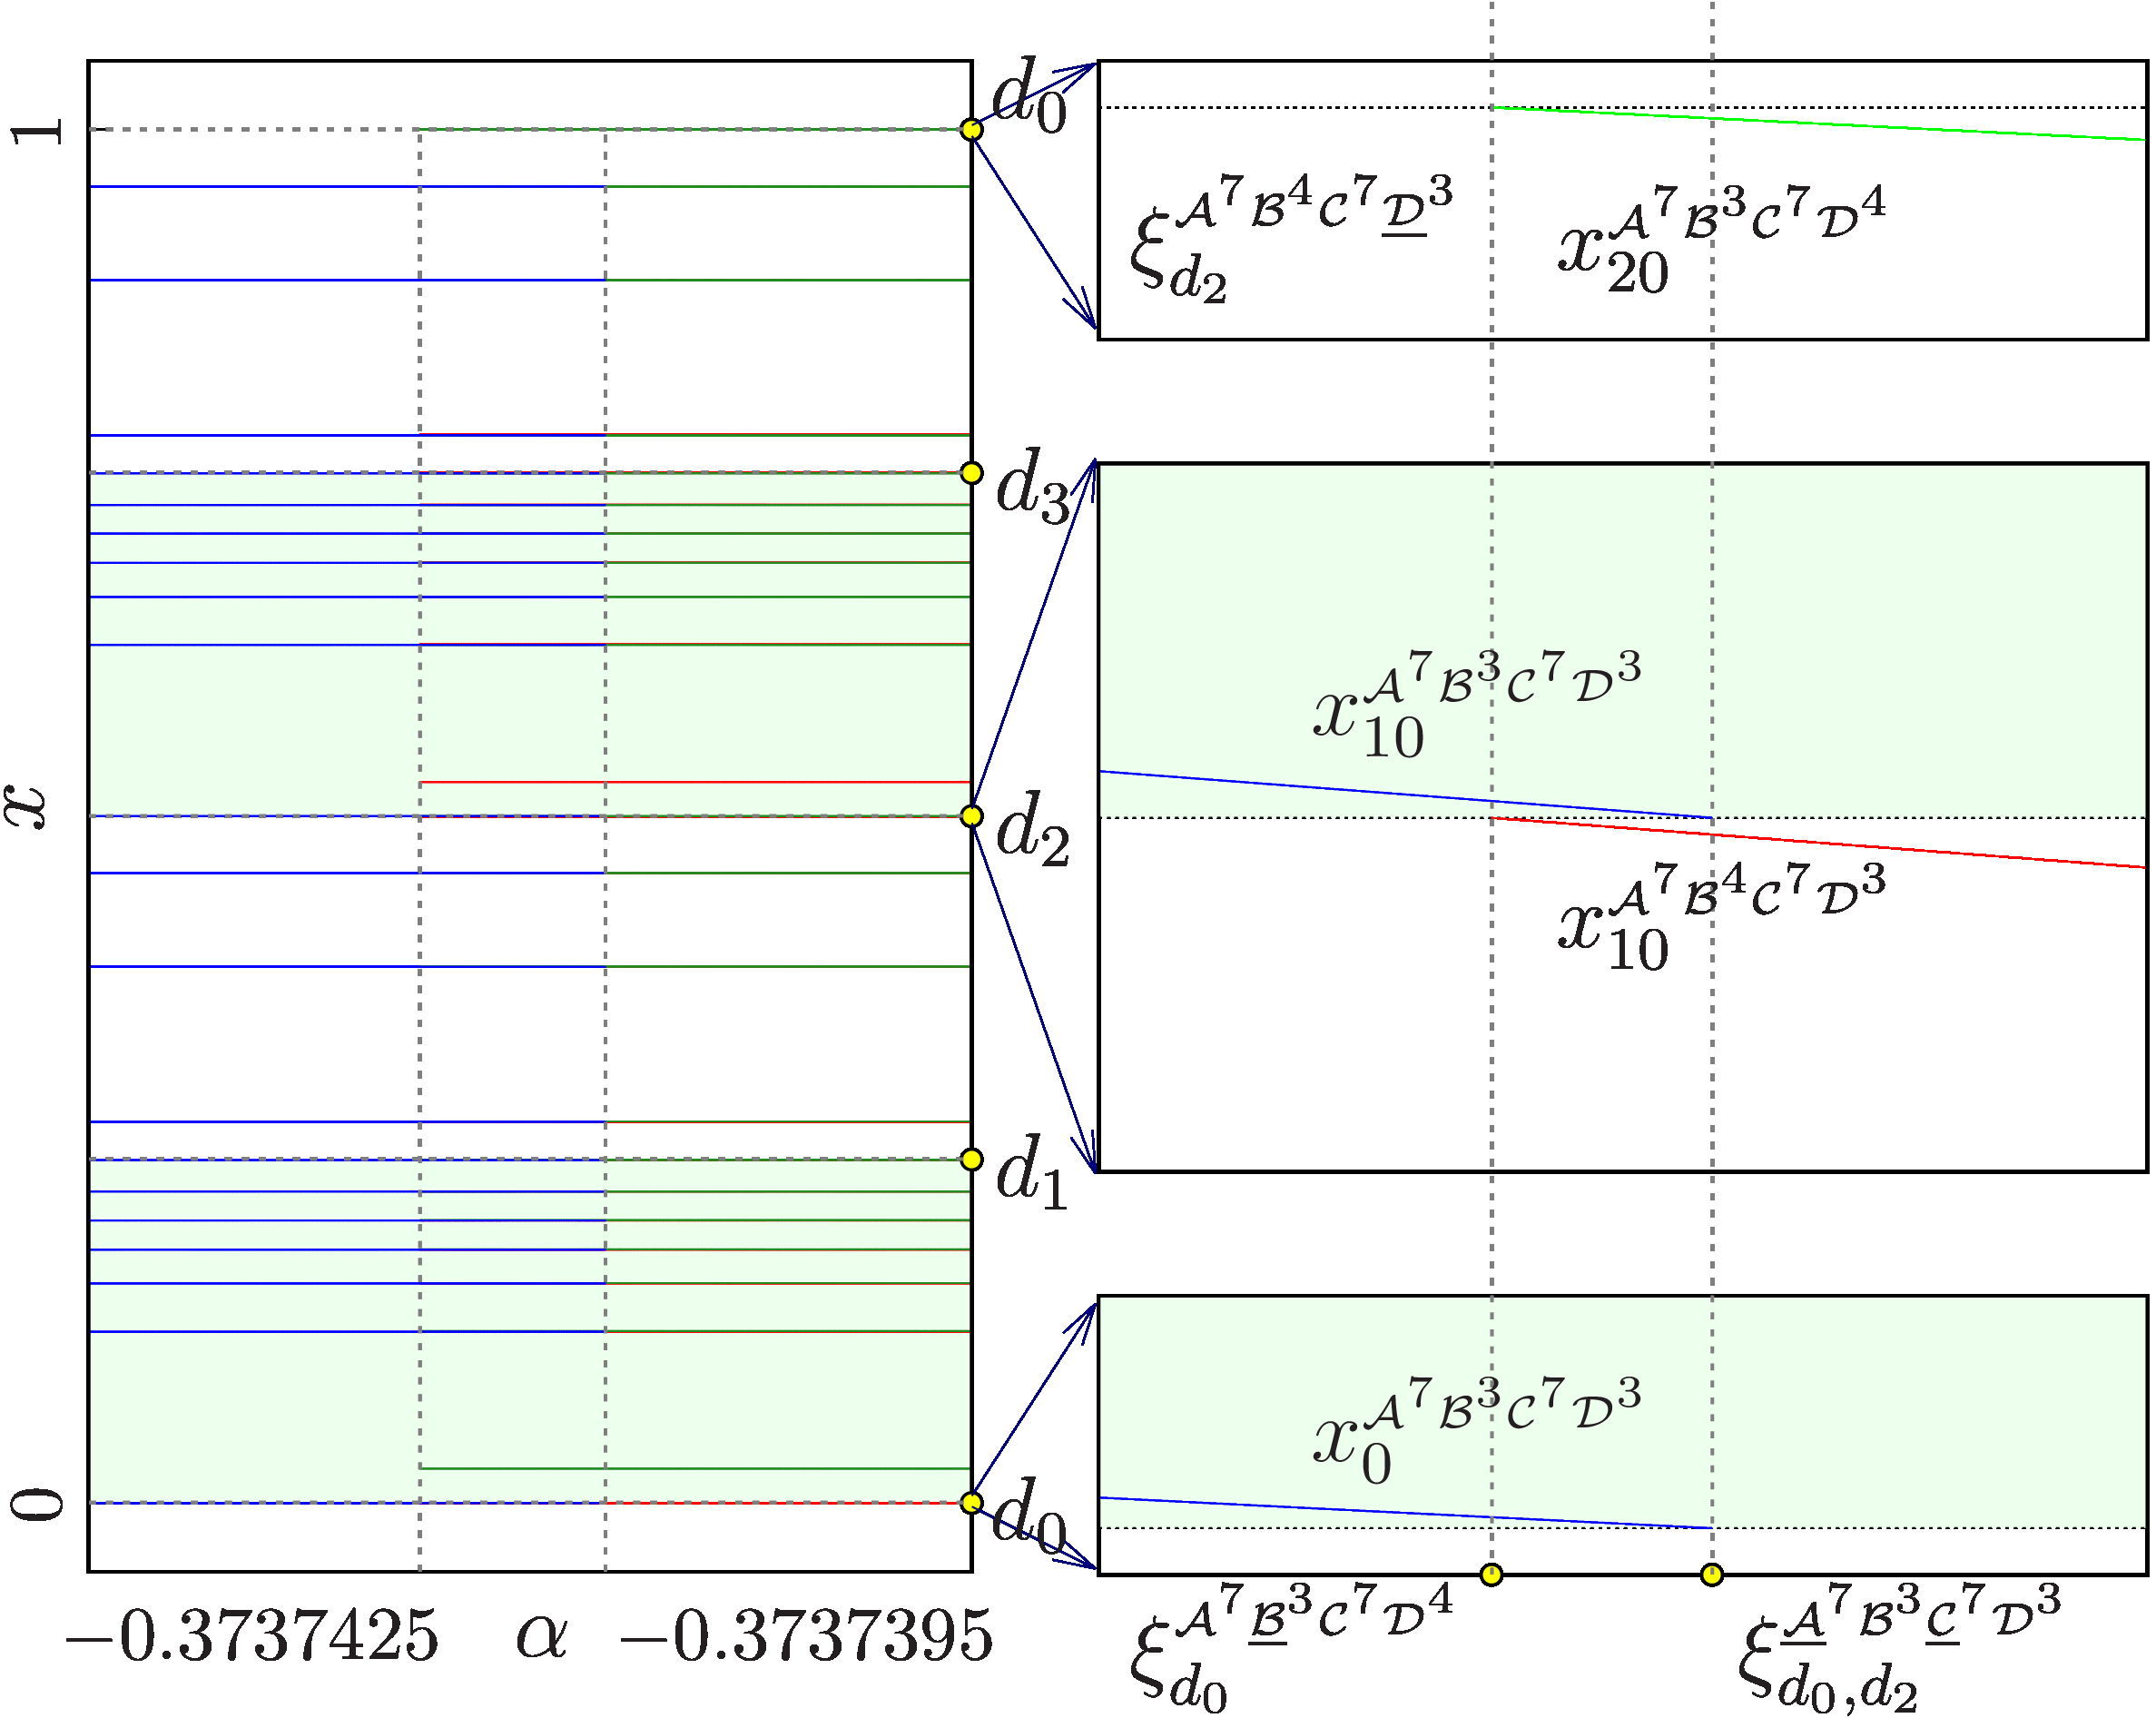
\includegraphics[width=.45 \textwidth]{../Figures/7/7.8a/result.png}
		\label{fig:add.appa.vert.bif.left}
	}
	\subfloat[Right boundary]{
		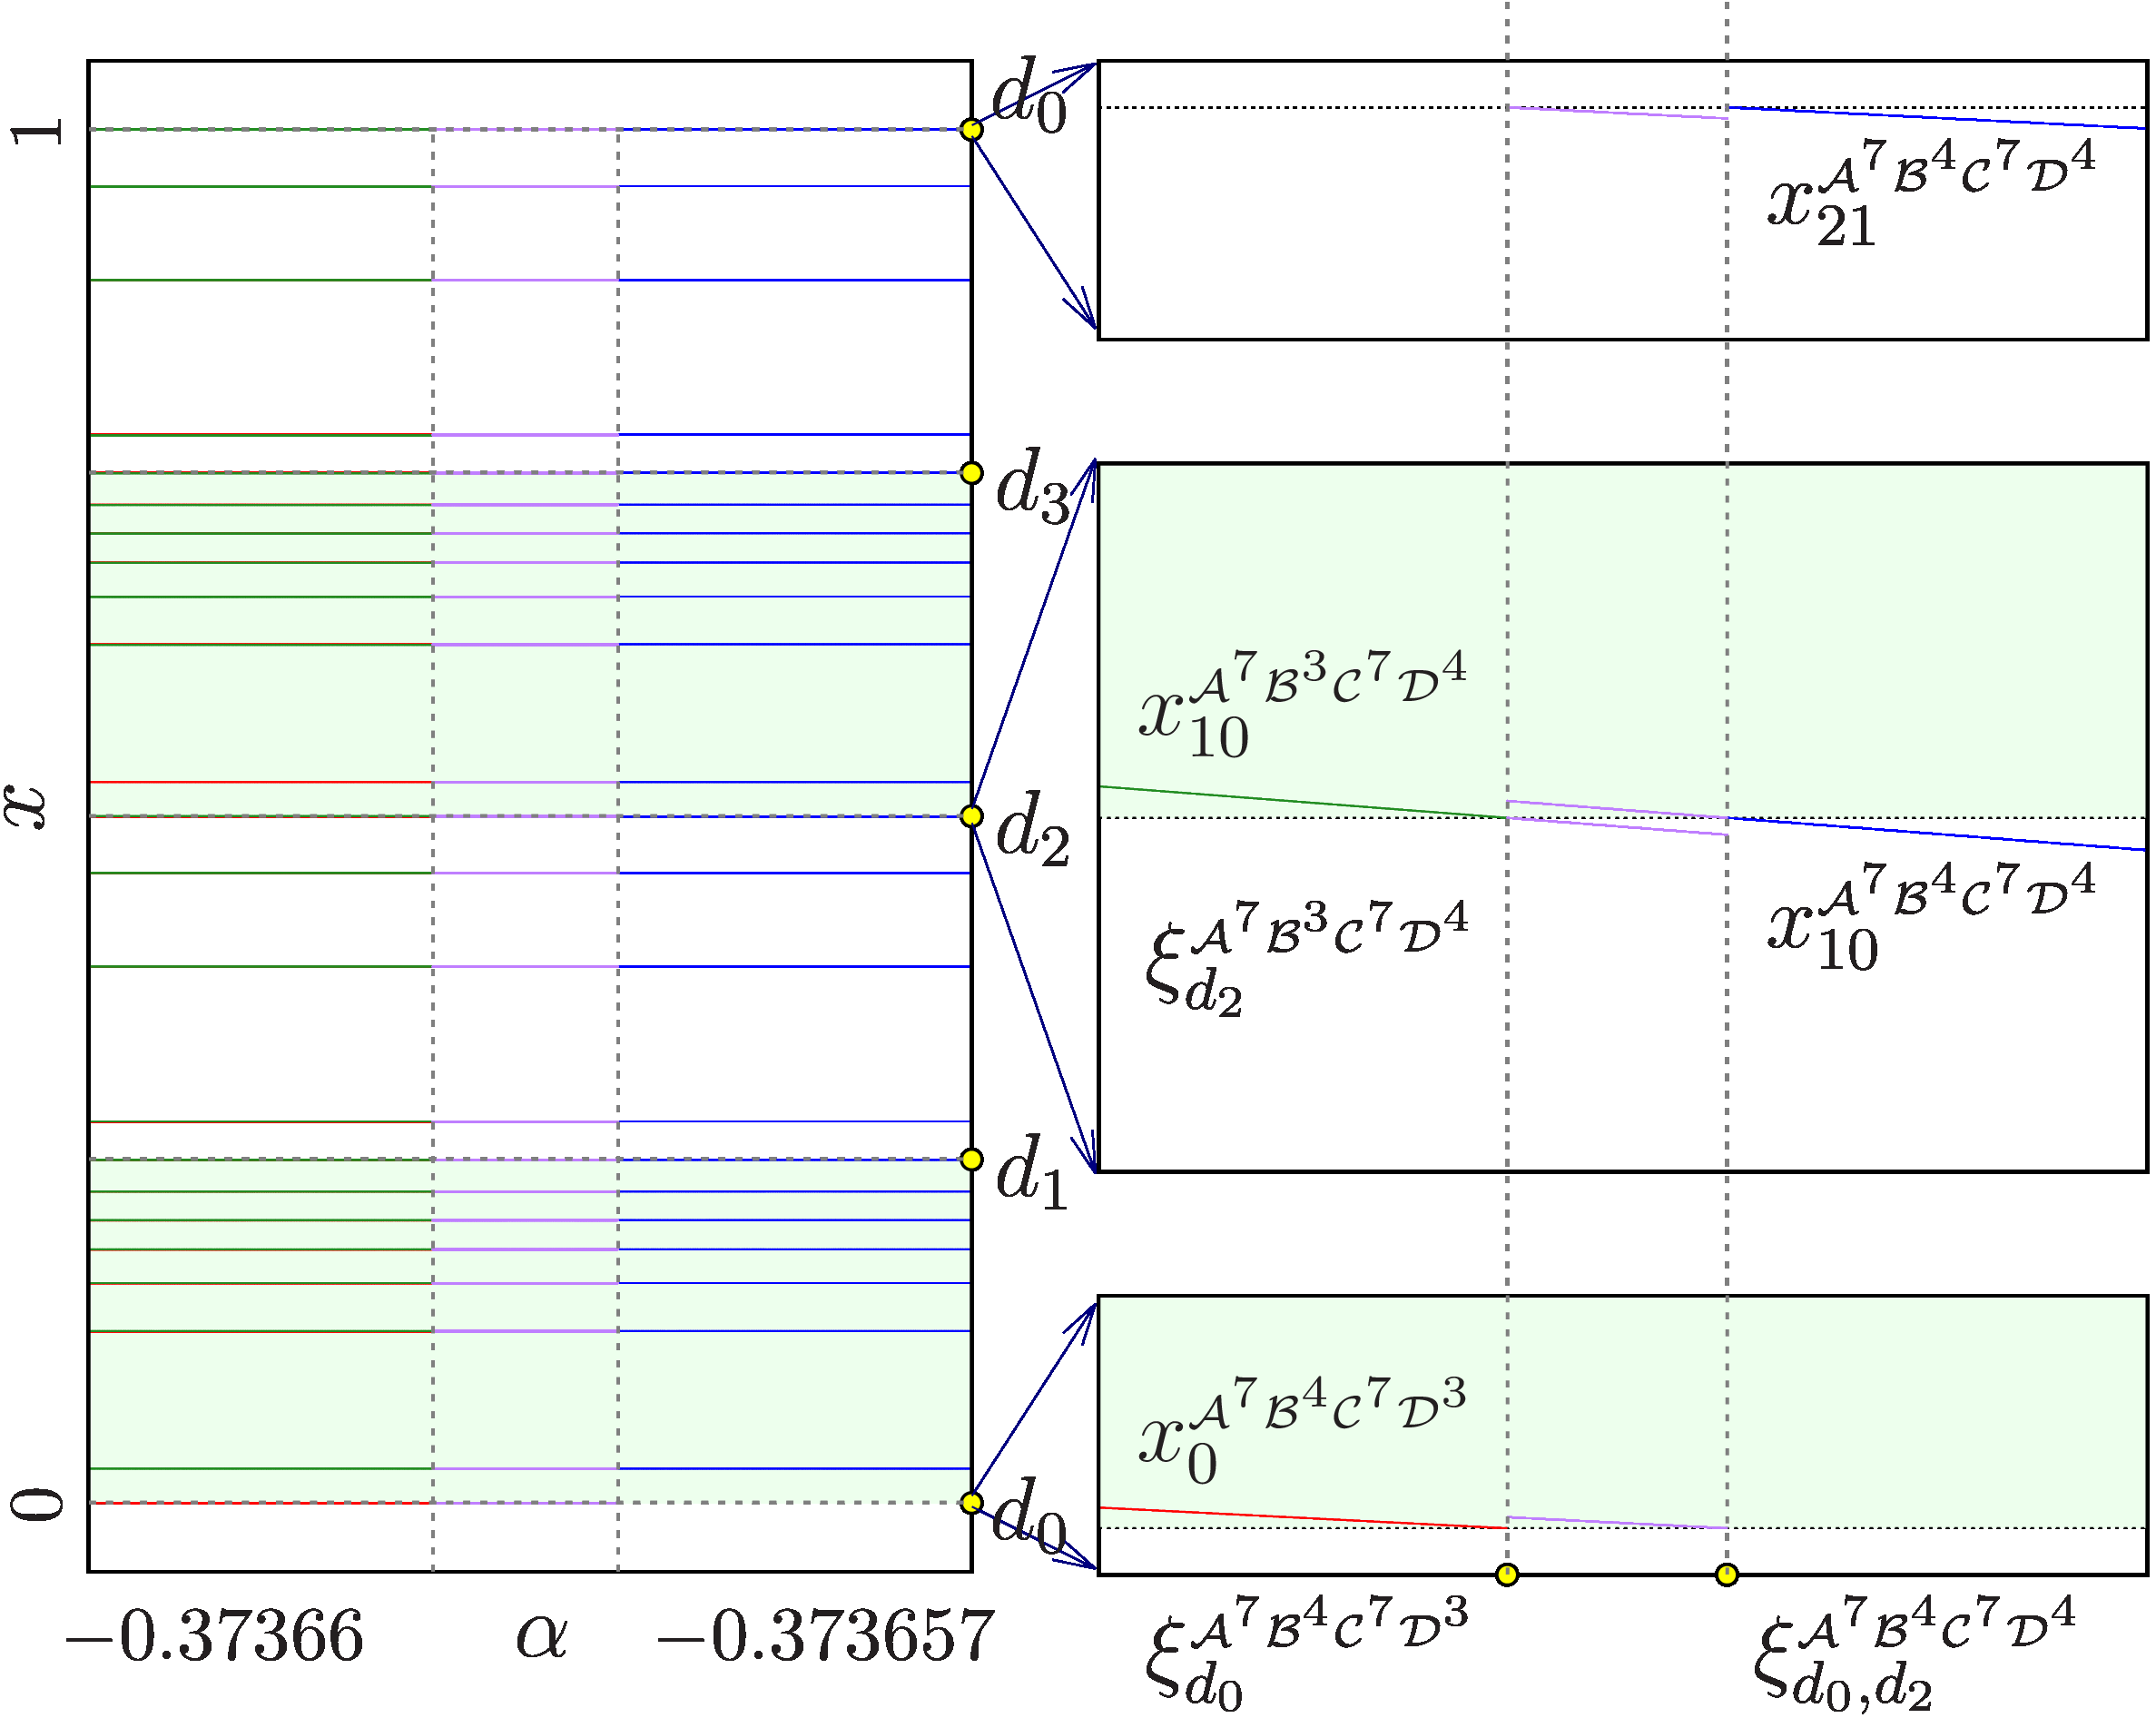
\includegraphics[width=.45 \textwidth]{../Figures/7/7.8b/result.png}
		\label{fig:add.appa.vert.bif.right}
	}
	\caption[Bifurcation diagrams for the vertical hybrid parameter regions in the increasing archetypal model]{
		Bifurcation diagrams at the vertical boundaries of the vertical hybrid parameter region $\left[P^{22}_4 \mid P^{20}_4\right]$.
		The parameters $a_L = 2.65, b_L = -0.05, g_R\left(\frac{1}{2}\right) = \frac{1}{2} + \frac{1}{40},$ and $\beta = c_L = 0.124797$ are fixed.
		The parameter $\alpha = g_R\left(\frac{1}{4}\right)$ is varied.
		(a) shows the bifurcation diagram at the left boundary, while (b) shows the bifurcation diagram at the right boundary.
	}
	\label{fig:add.appa.vert.bif}
\end{figure}
